
\documentclass[11pt,a4paper]{article}
\usepackage[utf8]{inputenc}
\usepackage[T1]{fontenc}
\usepackage[spanish,es-noshorthands,es-tabla,es-nodecimaldot]{babel}
\usepackage{lmodern}


\usepackage[a4paper,top=2.0cm,bottom=2.0cm,left=1.9cm,right=1.9cm,
            headheight=14pt,footskip=0.9cm]{geometry}

\usepackage{amsmath,amssymb}
\usepackage{bm}
\usepackage{graphicx}
\usepackage{xcolor}
\usepackage{booktabs}
\usepackage{tabularx}
\usepackage{array}
\usepackage{longtable}
\usepackage{enumitem}
\usepackage{fancyhdr}
\usepackage{titlesec}
\usepackage{listings}
\usepackage[most]{tcolorbox}
\usepackage{hyperref}
\usepackage[section]{placeins}
\usepackage{multicol}

% Optimización de colocación de flotantes para evitar páginas vacías
\renewcommand{\topfraction}{0.90}
\renewcommand{\bottomfraction}{0.90}
\renewcommand{\textfraction}{0.10}
\renewcommand{\floatpagefraction}{0.75}
\setlength{\floatsep}{6pt plus 2pt minus 2pt}
\setlength{\textfloatsep}{8pt plus 2pt minus 3pt}
\setlength{\intextsep}{6pt plus 2pt minus 2pt}

\definecolor{navy}{HTML}{1E2761}
\definecolor{coral}{HTML}{F96167}
\definecolor{iceblue}{HTML}{CADCFC}
\definecolor{grisclaro}{HTML}{F4F6FB}

\hypersetup{
  colorlinks=true,
  linkcolor=navy,
  urlcolor=coral,
  citecolor=navy,
  pdftitle={Laboratorio 1 - Logica CMOS estatica},
  pdfauthor={MsC. Luz Adanaque Infante - UNMSM FIEE}
}

%------------------------------ Encabezados ----------------------------------
\pagestyle{fancy}
\fancyhf{}
\fancyhead[L]{\footnotesize\color{navy}\textsc{Microelectrónica} · Laboratorio N.\textsuperscript{o} 1}
\fancyhead[R]{\footnotesize\color{navy}Lógica CMOS estática}
\fancyfoot[L]{\footnotesize\color{navy}MsC. Luz Adanaqué Infante}
\fancyfoot[C]{\footnotesize\color{navy}UNMSM -- FIEE}
\fancyfoot[R]{\footnotesize\color{navy}\thepage}
\renewcommand{\headrulewidth}{0.8pt}
\renewcommand{\footrulewidth}{0.4pt}
\renewcommand{\headrule}{\hbox to\headwidth{\color{coral}\leaders\hrule height \headrulewidth\hfill}}

%------------------------------ Titulos --------------------------------------
\titleformat{\section}
  {\normalfont\Large\bfseries\color{navy}}{\thesection.}{0.6em}{}
  [\vspace{-0.6em}{\color{coral}\rule{\textwidth}{1.2pt}}]
\titleformat{\subsection}
  {\normalfont\large\bfseries\color{navy}}{\thesubsection}{0.6em}{}
\titlespacing*{\section}{0pt}{1.0em}{0.4em}
\titlespacing*{\subsection}{0pt}{0.7em}{0.3em}

%------------------------- Estilo para codigo SPICE --------------------------
\lstdefinelanguage{SPICE}{
  alsoletter={.},
  morekeywords={.include,.param,.model,.tran,.dc,.ac,.op,.meas,.measure,.step,
                .ic,.subckt,.ends,.end,.options,.lib,.save,.four,
                PULSE,PWL,SIN,TRIG,TARG,VAL,RISE,FALL,TD,AVG,MAX,MIN,PARAM,
                FIND,WHEN,AT,DERIV,nmos,pmos,level},
  sensitive=false,
  morecomment=[f]{*},
  morecomment=[l]{;},
}
\lstdefinestyle{spice}{
  language=SPICE,
  basicstyle=\ttfamily\scriptsize,
  keywordstyle=\color{navy}\bfseries,
  commentstyle=\color{coral!85!black}\itshape,
  backgroundcolor=\color{grisclaro},
  frame=leftline,
  framerule=1.5pt,
  rulecolor=\color{iceblue},
  framesep=4pt,
  xleftmargin=6pt,
  breaklines=true,
  showstringspaces=false,
  columns=fullflexible,
  aboveskip=0.4em,
  belowskip=0.4em,
}
\lstset{style=spice}

%------------------------------- Cajas ---------------------------------------
\newtcolorbox{aviso}[1][]{
  enhanced, breakable, colback=coral!8, colframe=coral,
  boxrule=0pt, leftrule=3.5pt, arc=2pt, left=6pt, right=6pt, top=4pt, bottom=4pt,
  fonttitle=\bfseries\color{white}, #1}

\newtcolorbox{nota}[1][]{
  enhanced, breakable, colback=iceblue!35, colframe=navy,
  boxrule=0pt, leftrule=3.5pt, arc=2pt, left=6pt, right=6pt, top=4pt, bottom=4pt,
  #1}

\newtcolorbox{preguntas}[1][]{
  enhanced, breakable, colback=white, colframe=navy,
  boxrule=0.8pt, arc=2pt, left=6pt, right=6pt, top=4pt, bottom=4pt,
  title={\bfseries #1}, coltitle=white, colbacktitle=navy}

%------------------------- Contador de preguntas -----------------------------
\newcounter{preg}
\newcommand{\preg}[1]{\refstepcounter{preg}\item[\textbf{\color{coral}P\thepreg.}] #1}
\newenvironment{listapreg}{\begin{list}{}{%
  \setlength{\leftmargin}{1.8em}\setlength{\labelwidth}{1.6em}%
  \setlength{\itemsep}{0.25em}\setlength{\parsep}{0pt}}}{\end{list}}

%------------------------------ Utilidades -----------------------------------
\newcommand{\vacio}{\rule[-1.4ex]{0pt}{4.2ex}}
\renewcommand{\arraystretch}{1.12}
\setlength{\tabcolsep}{4pt}

%==============================================================================
\begin{document}
%==============================================================================

%------------------------------- Portada -------------------------------------
\begin{titlepage}
\centering
\vspace*{1.2cm}

{\color{navy}\rule{\textwidth}{2pt}}\\[0.5em]
{\Large\bfseries\color{navy} UNIVERSIDAD NACIONAL MAYOR DE SAN MARCOS}\\[0.35em]
{\normalsize\color{navy} Universidad del Perú, Decana de América}\\[0.6em]
{\color{coral}\rule{\textwidth}{2pt}}\\[1.4cm]


{\large\color{navy} Facultad de Ingeniería Electrónica y Eléctrica}\\[0.3em]
{\large\color{navy} Escuela Profesional de Ingeniería Electrónica}\\[2.2cm]

{\color{coral}\Large\bfseries GUÍA DE LABORATORIO N.\textsuperscript{o} 1}\\[0.9cm]
{\Huge\bfseries\color{navy} Lógica CMOS Estática}\\[0.7cm]
{\large\color{navy}\itshape Caracterización, dimensionamiento y potencia\\ con modelos predictivos PTM en LTspice}\\[2.4cm]

\begin{tabular}{@{}r@{\hspace{1em}}l@{}}
\bfseries\color{navy} Curso: & Microelectrónica \\
\bfseries\color{navy} Unidad: & Modelamiento de circuitos \\
\bfseries\color{navy} Docente: & MsC. Luz Adanaqué Infante \\
\bfseries\color{navy} Integrantes: & Leonardo Sait Yactayo Tolentino (23190214) \\
                                   & Marco Antonio Arcila Santander (23190140) \\
\bfseries\color{navy} Modalidad: & Parejas \\
\end{tabular}

\vfill
{\color{iceblue}\rule{\textwidth}{6pt}}\\[0.4em]
{\footnotesize\color{navy} Lima, Perú}
\end{titlepage}

%--------------------------------- Indice ------------------------------------
{\color{navy}\tableofcontents}
\vspace{1.5em}

%==============================================================================
\section{Objetivos}
%==============================================================================

Al terminar la sesión el estudiante será capaz de:

\begin{enumerate}[leftmargin=1.6em,itemsep=0.35em]
  \item Configurar un entorno de simulación con tarjetas de modelo predictivas (PTM) para distintos nodos tecnológicos.
  \item Extraer la curva de transferencia (VTC) de un inversor CMOS estático y determinar $V_M$, $V_{IL}$, $V_{IH}$ y los márgenes de ruido.

  \item Medir retardos de propagación, tiempos de transición y su dependencia con la carga y el nodo tecnológico.
  \item Sintetizar compuertas complejas (NAND, NOR, AOI) mediante redes pull-up / pull-down duales y verificarlas funcionalmente.
  \item Cuantificar las tres componentes de potencia (dinámica, cortocircuito y fuga) y contrastar procesos HP frente a LP.
\end{enumerate}

%==============================================================================
\section{Fundamento resumido y Pre-lab}
%==============================================================================

La lógica CMOS estática implementa una función lógica $Y = \overline{F(A,B,\dots)}$ mediante dos redes complementarias: una red \emph{pull-down} (PDN) de transistores NMOS que conduce hacia tierra cuando $F=1$, y una red \emph{pull-up} (PUN) de transistores PMOS, grafo dual de la anterior, que conmuta hacia $V_{DD}$ cuando $F=0$. En régimen estático solo una de las dos redes conduce plenamente, de modo que en el modelo ideal no existe camino DC entre $V_{DD}$ y tierra ($I_{DC} \approx 0$).

\subsection*{Deducción analítica del punto de conmutación $V_M$ (Pre-lab)}

El punto de conmutación o umbral lógico $V_M$ se define como el punto de la característica de transferencia de tensión (VTC) donde el voltaje de salida iguala al voltaje de entrada:
\begin{equation}
V_{in} = V_{out} = V_M
\label{eq:cond_vm}
\end{equation}

\noindent\textbf{1. Hipótesis operativas y modelo físico de saturación:}\\
En un inversor CMOS nanométrico (Figura~\ref{fig:esquema_inv}), se establecen las siguientes condiciones de partida:
\begin{enumerate}[leftmargin=1.4em,itemsep=0.15em]
  \item \emph{Geometría de canal mínimo:} Se adopta la misma longitud dibujada de canal para ambos dispositivos, $L_n = L_p = L_{\min} = 45\text{~nm}$, optimizando el área de integración.
  \item \emph{Potenciales de sustrato (Bulk):} Ambos transistores tienen su sustrato conectado a su respectiva fuente ($V_{SBn} = 0$, $V_{SBp} = 0$), anulando la modulación del potencial de canal por efecto cuerpo ($\gamma = 0$ y $\Delta V_T = 0$), lo que fija $V_{Tn} = V_{TH0,n}$ y $V_{Tp} = V_{TH0,p}$ (con la convención $V_{Tp} < 0$).
  \item \emph{Saturación por velocidad de deriva extrema:} El modelo por tramos de canal corto establece que la corriente en saturación de velocidad es $I_D = W C_{ox} v_{sat} (V_{GS} - V_T - V_{DSAT}/2)$. Bajo fuerte campo longitudinal ($\mathcal{E} \gg \mathcal{E}_{sat}$), la sobretensión de compuerta supera holgadamente la caída de saturación ($(V_{GS} - V_T) \gg V_{DSAT}/2$), permitiendo aproximar la corriente con una dependencia lineal directa respecto a la sobretensión:
  \begin{equation}
  I_D \approx k\,V_{DSAT}\,(V_{GS} - V_T) = W\,C_{ox}\,v_{sat}\,(V_{GS} - V_T)
  \label{eq:id_sat}
  \end{equation}
  donde $k = \mu\,C_{ox}\frac{W}{L}$ y la velocidad de saturación límite cumple $v_{sat} = \mu\,\mathcal{E}_{sat} = \mu \frac{V_{DSAT}}{L}$. De aquí se desprende la identidad fundamental $k\,V_{DSAT} = C_{ox}\,W\,v_{sat}$, válida al ser $L_n = L_p = L_{\min}$.
\end{enumerate}

\noindent\textbf{2. Equilibrio estático de corrientes:}\\
Al no existir corriente de compuerta estacionaria hacia la carga ($I_{out} = 0$), la corriente que drena el PMOS debe igualar exactamente a la que absorbe el NMOS ($I_{Dn} = I_{Dp}$):
\begin{align}
I_{Dn} &= k_n\,V_{DSATn}\,(V_{GSn} - V_{Tn}) = k_n\,V_{DSATn}\,(V_M - V_{Tn}) \label{eq:idn}\\
I_{Dp} &= k_p\,V_{DSATp}\,(V_{SGp} - |V_{Tp}|) = k_p\,V_{DSATp}\,(V_{DD} - V_M + V_{Tp}) \label{eq:idp}
\end{align}
donde se emplea $-|V_{Tp}| = +V_{Tp}$ ($V_{Tp} < 0$). Igualando~\eqref{eq:idn} y~\eqref{eq:idp} y definiendo la razón de transconductancia de saturación $r$:
\begin{equation}
r \equiv \frac{k_p\,V_{DSATp}}{k_n\,V_{DSATn}} = \frac{C_{ox}\,W_p\,v_{sat,p}}{C_{ox}\,W_n\,v_{sat,n}} = \frac{W_p}{W_n}\cdot\frac{v_{sat,p}}{v_{sat,n}} = \beta\cdot\frac{v_{sat,p}}{v_{sat,n}}
\label{eq:r_def}
\end{equation}
donde $\beta \equiv W_p / W_n$. Sustituyendo $r$ en la igualdad $I_{Dn} = I_{Dp}$:
\begin{equation}
V_M - V_{Tn} = r\,\left(V_{DD} - V_M + V_{Tp}\right) \implies V_M\,(1 + r) = V_{Tn} + r\,(V_{DD} + V_{Tp})
\end{equation}
Despejando analíticamente, se llega a la expresión gobernante del umbral lógico:
\begin{equation}
V_M = \frac{V_{Tn} + r\,(V_{DD}+V_{Tp})}{1+r}, \qquad r = \beta\cdot\frac{v_{sat,p}}{v_{sat,n}}
\label{eq:vm}
\end{equation}

\noindent\textbf{3. Condición de dimensionamiento para centrado simétrico ($V_M = V_{DD}/2$):}\\
Para maximizar y equilibrar simétricamente los márgenes de ruido ($NM_L = NM_H$), se impone $V_M = V_{DD}/2$:
\begin{equation}
\frac{V_{DD}}{2} = \frac{V_{Tn} + r\,(V_{DD} + V_{Tp})}{1 + r} \implies r = \frac{\frac{V_{DD}}{2} - V_{Tn}}{\frac{V_{DD}}{2} - |V_{Tp}|}
\end{equation}
Sustituyendo la definición $r = \beta\,(v_{sat,p}/v_{sat,n})$, se deduce el factor de aspecto óptimo de diseño $\beta_{\text{sim}}$:
\begin{equation}
\beta_{\text{sim}} = \left(\frac{\frac{V_{DD}}{2} - V_{Tn}}{\frac{V_{DD}}{2} - |V_{Tp}|}\right) \cdot \frac{v_{sat,n}}{v_{sat,p}}
\label{eq:beta_opt}
\end{equation}
Bajo umbrales aproximadamente simétricos ($V_{Tn} \approx |V_{Tp}|$), la razón exige $r \approx 1$, lo que impone la condición directa $\beta_{\text{sim}} \approx v_{sat,n}/v_{sat,p}$. A diferencia de canal largo (donde la regla clásica predice $\beta \approx \mu_n/\mu_p \approx 2.70$), en nodos nanométricos sub-65~nm el centrado queda dominado por la razón de velocidades de saturación ($v_{sat,n}/v_{sat,p} \approx 1.13$), convergiendo en la simulación a $\beta \approx 2.50$ debido a los efectos combinados de canal corto.

\noindent\textbf{4. Condiciones de borde para saturación simultánea:}\\
Para garantizar la validez física de la deducción, ambos dispositivos deben operar efectivamente en saturación en $V_{in} = V_{out} = V_M$:
\begin{equation}
V_{DSn} = V_M \ge V_{DSATn} \qquad\text{y}\qquad V_{SDp} = (V_{DD} - V_M) \ge V_{DSATp}
\label{eq:cond_sat}
\end{equation}
En la tecnología 45~nm HP ($V_{DD}=1.0\text{~V}$, $V_{DSATn} \approx 0.12\text{~V}$, $V_{DSATp} \approx 0.15\text{~V}$), al encontrarse $V_M \approx 0.50\text{~V}$, se cumple $0.50\text{~V} \ge 0.12\text{~V}$ y $0.50\text{~V} \ge 0.15\text{~V}$ con amplio margen, asegurando la rigurosa estabilidad del punto de operación.

\begin{figure}[htbp]
\centering
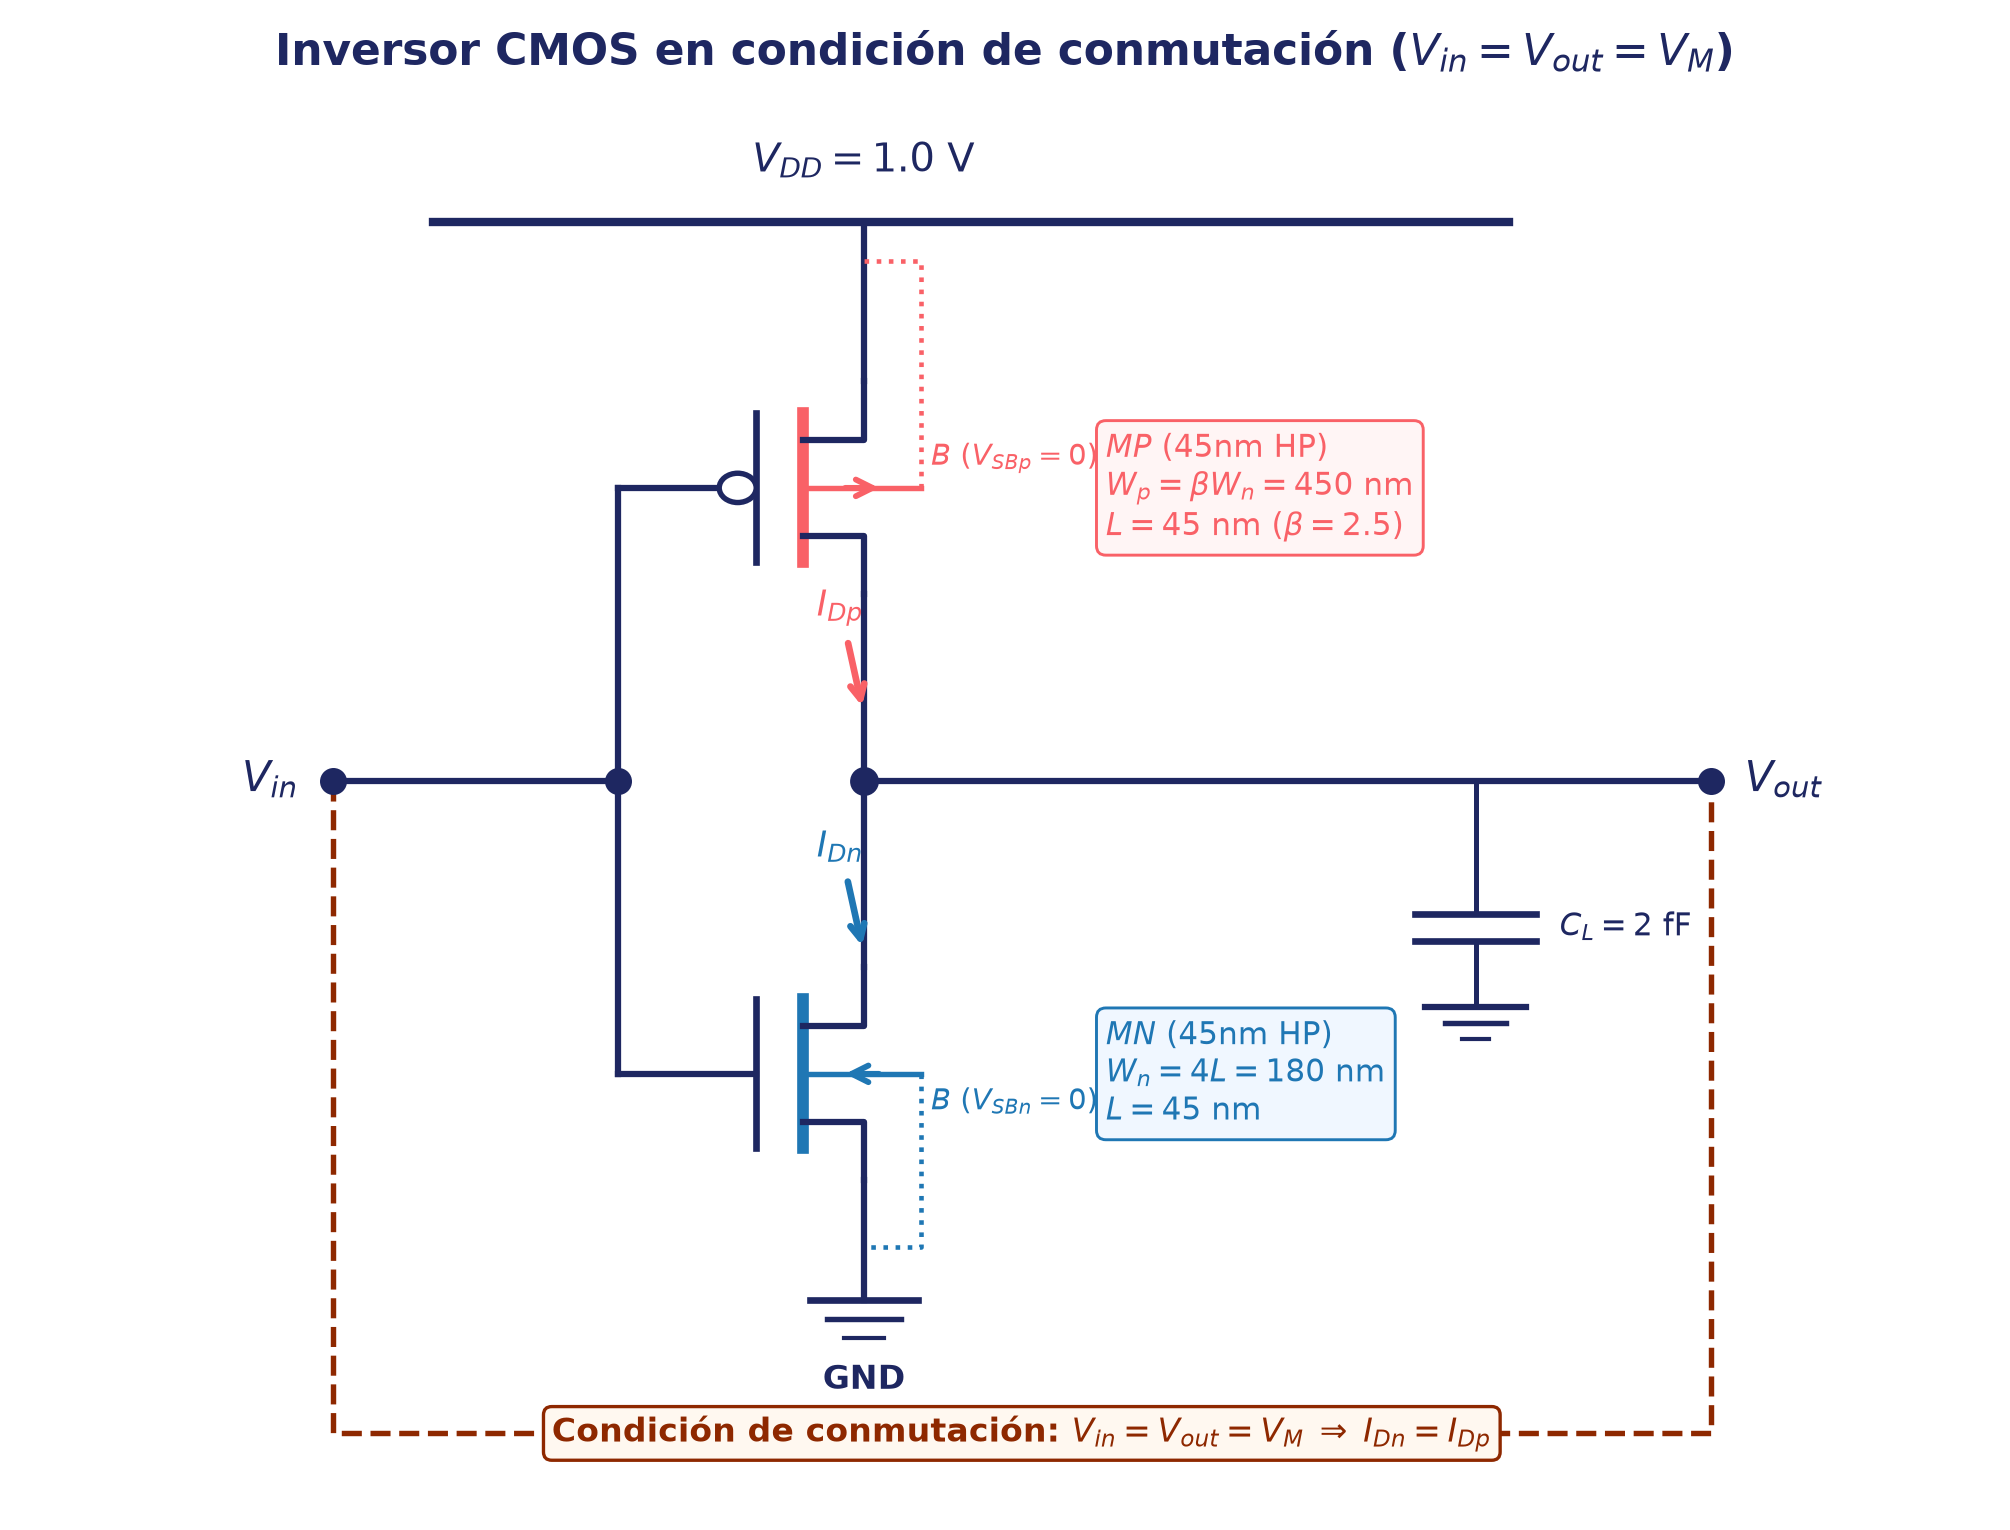
\includegraphics[width=0.48\textwidth,height=4.8cm,keepaspectratio]{figuras/fig_esquema_inversor.png}
\caption{Esquema circuital del inversor CMOS (45~nm HP) en condición de conmutación ($V_{in} = V_{out} = V_M$, $I_{Dn} = I_{Dp}$), explicitando terminales de sustrato ($V_{SB}=0$), polarización, carga $C_L=2$~fF y parámetros de diseño.}
\label{fig:esquema_inv}
\end{figure}
\FloatBarrier

\subsection*{Dinámica de retardo y componentes de potencia}

\paragraph{Retardo de propagación y descomposición capacitiva.}
El retardo medio de propagación $t_p$ se define como el promedio entre los tiempos de respuesta de subida y bajada:
\begin{equation}
t_p = \tfrac{1}{2}\left(t_{pHL}+t_{pLH}\right), \qquad t_{pHL} \approx 0.69\,R_{eq,n}\,C_L, \qquad t_{pLH} \approx 0.69\,R_{eq,p}\,C_L
\label{eq:tp}
\end{equation}
donde las resistencias efectivas de canal cumplen $R_{eq,n} \propto \frac{1}{W_n}$ y $R_{eq,p} \propto \frac{1}{W_p} = \frac{1}{\beta W_n}$. En un circuito integrado, la capacitancia total del nodo de conmutación $C_L$ no es meramente una carga concentrada externa, sino la superposición de componentes parásitas intrínsecas y de carga:
\begin{equation}
C_L = C_{ext} + C_{int} = C_{ext} + \underbrace{(C_{db,n} + C_{db,p})}_{\text{difusión}} + \underbrace{(C_{gd,n} + C_{gd,p})}_{\text{solapamiento}} + C_{wire}
\label{eq:cl_split}
\end{equation}
Esta descomposición justifica físicamente por qué en la recta $t_p(C_L) = m\,C_L + t_0$, la ordenada al origen no es nula: $t_0 \approx 0.69\,R_{eq}\,C_{int}$ modela el retardo intrínseco descargado.

\paragraph{Disipación de potencia total.}
La potencia consumida por el inversor en conmutación periódica a frecuencia $f$ con factor de actividad $\alpha$ se modela mediante sus tres componentes fundamentales:
\begin{equation}
P_{tot} = \underbrace{\alpha\,C_L V_{DD}^{2} f}_{\text{dinámica de conmutación}}
        + \underbrace{I_{cc}\,V_{DD}}_{\text{cortocircuito en transición}}
        + \underbrace{I_{leak}\,V_{DD}}_{\text{fuga estática}}
\label{eq:pot}
\end{equation}


\section{Entorno y Modelos Tecnológicos}

Las simulaciones fueron implementadas en LTspice 24 utilizando las tarjetas del \emph{Predictive Technology Model} (PTM, Arizona State University) correspondientes a los nodos de 90~nm bulk, 45~nm (procesos HP y LP) y 22~nm HP bajo la formulación BSIM4 (nivel 54 / 14 en LTspice). 

Para los análisis de caracterización y contraste entre procesos, se implementaron librerías con renombramiento de modelos (\texttt{45nm\_HP\_ren.lib} y \texttt{45nm\_LP\_ren.lib}) asignando identificadores unívocos (\texttt{nmos\_45hp}, \texttt{pmos\_45hp}, \texttt{nmos\_45lp}, \texttt{pmos\_45lp}), mitigando la sobreescritura silenciosa de modelos en directivas \lstinline|.include|. A lo largo del informe se adopta un ancho de referencia $W_n = 4L$ como transistor unitario y longitudes de canal nominales fijadas por cada nodo tecnológico.

%==============================================================================
\section{Actividad 1 --- Inversor CMOS: VTC y márgenes de ruido}
%==============================================================================

\subsection*{Procedimiento}
\begin{enumerate}[leftmargin=1.6em,itemsep=0.35em]
  \item Arme el circuito del Anexo~\ref{sec:a1} con la tarjeta de 45~nm HP, $V_{DD}=1.0$~V, $L=45$~nm, $W_n=180$~nm.
  \item Ejecute el barrido DC con \lstinline|.step param beta 1 3 0.5| y grafique la familia de curvas $V_{out}(V_{in})$.
  \item Registre $V_M$ para cada valor de $\beta$ mediante la directiva \lstinline|.meas|. Los resultados se leen en el archivo de registro (\texttt{Ctrl+L}).
  \item Para el caso de $\beta$ que hace $V_M \approx V_{DD}/2$: grafique la derivada \lstinline|d(V(out))| en el visor de formas de onda y ubique con cursores los dos puntos donde la pendiente vale $-1$. Esos son $V_{IL}$ y $V_{IH}$.
  \item Calcule $NM_H = V_{OH}-V_{IH}$ y $NM_L = V_{IL}-V_{OL}$.
\end{enumerate}

\begin{table}[htbp]
\centering\small
\caption{Resultados 1.1 --- Barrido de la razón $\beta$.}
\label{tab:res11}
\begin{tabularx}{\textwidth}{@{}c*{6}{>{\centering\arraybackslash}X}@{}}
\toprule
$\bm{\beta}$ & $\bm{V_M}$ (V) & $\bm{V_{IL}}$ (V) & $\bm{V_{IH}}$ (V) & $\bm{NM_L}$ (V) & $\bm{NM_H}$ (V) & \textbf{Gan. máx.} \\
\midrule
1.0 & 0.4632 & 0.3460 & 0.5560 & 0.3460 & 0.4440 & 6.18 \\
1.5 & 0.4791 & 0.3680 & 0.5760 & 0.3680 & 0.4240 & 6.13 \\
2.0 & 0.4903 & 0.3820 & 0.5920 & 0.3820 & 0.4080 & 6.10 \\
2.5 & 0.4989 & 0.3920 & 0.6040 & 0.3920 & 0.3960 & 6.08 \\
3.0 & 0.5058 & 0.4020 & 0.6140 & 0.4020 & 0.3860 & 6.06 \\
\bottomrule
\end{tabularx}
\end{table}

\begin{table}[htbp]
\centering\small
\caption{Resultados 1.2 --- Parámetros extraídos de \texttt{45nm\_HP.pm}.}
\label{tab:res12}
\begin{tabularx}{0.85\textwidth}{@{}l*{3}{>{\centering\arraybackslash}X}@{}}
\toprule
\textbf{Parámetro} & \textbf{NMOS} & \textbf{PMOS} & \textbf{Razón n/p} \\
\midrule
\texttt{u0} (movilidad) & 0.0540~m$^2$/V$\cdot$s & 0.0200~m$^2$/V$\cdot$s & 2.70 \\
\texttt{vsat}           & $1.70 \times 10^5$~m/s & $1.50 \times 10^5$~m/s & 1.13 \\
\texttt{vth0}           & 0.4689~V & $-0.4916$~V & 0.95 \\
\bottomrule
\end{tabularx}
\end{table}

\begin{figure}[htbp]
\centering
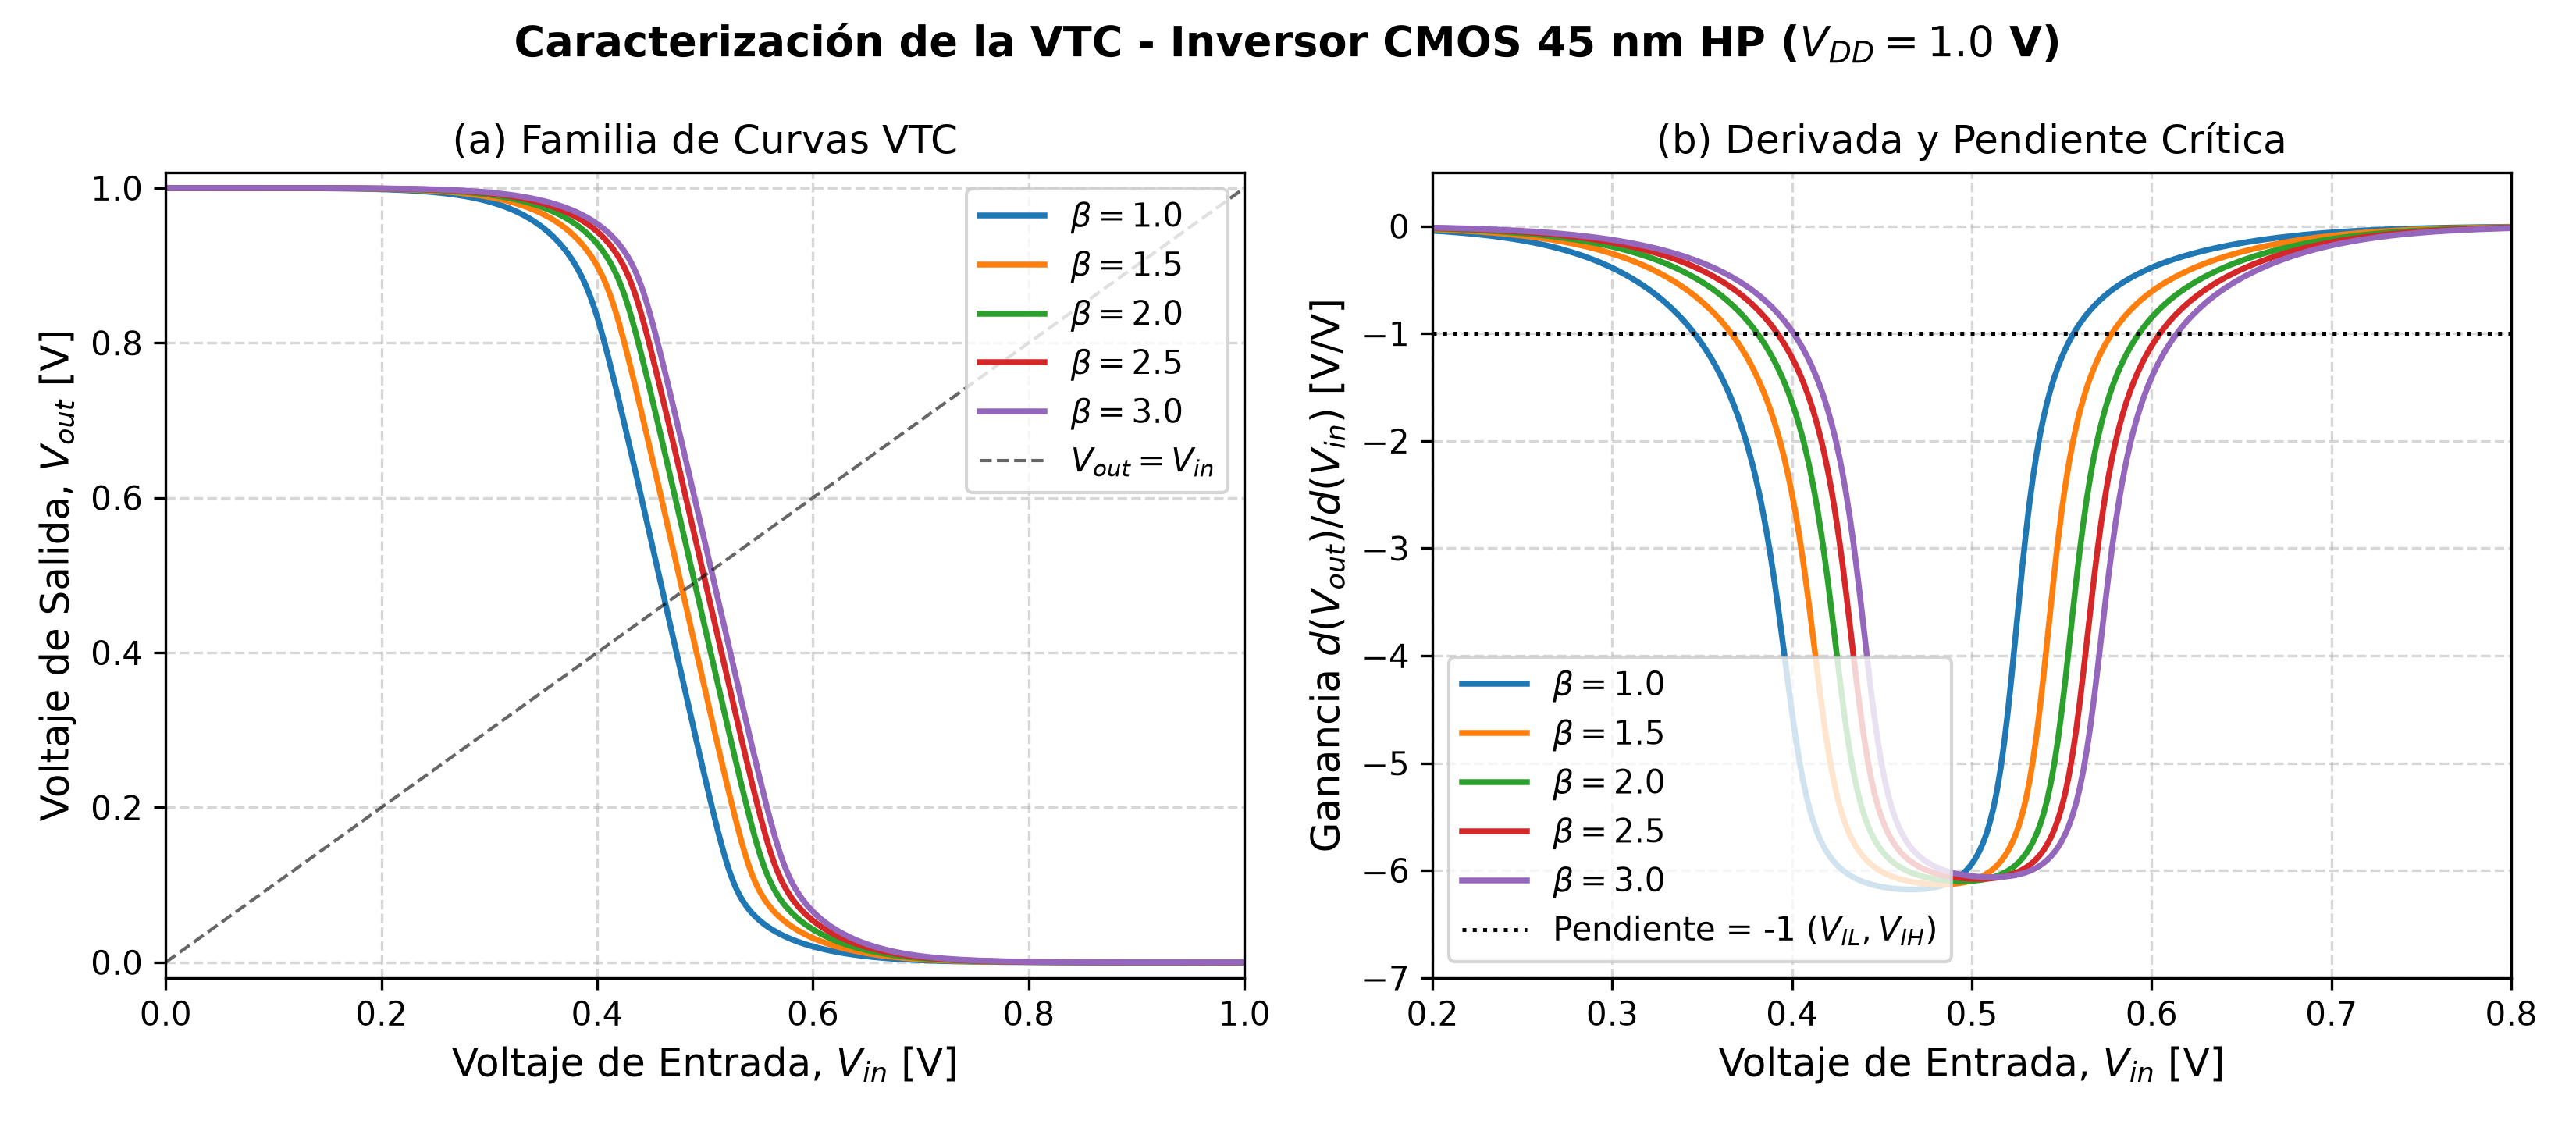
\includegraphics[width=0.72\textwidth,height=4.5cm,keepaspectratio]{figuras/fig1_vtc_familia.png}
\caption{Curvas de transferencia de voltaje (VTC) y derivada $d(V_{out})/d(V_{in})$ para el inversor CMOS de 45~nm HP ante el barrido de $\beta \in [1.0, 3.0]$. Se identifican los puntos de pendiente $-1$ ($V_{IL}, V_{IH}$) y el centrado en $\beta \approx 2.5$.}
\label{fig:vtc_familia}
\end{figure}
\FloatBarrier

\begin{preguntas}[Preguntas de la Actividad 1]
\begin{listapreg}
\preg{Con la razón de \texttt{u0} obtenida, la regla clásica predice cierto $\beta$ para centrar la VTC. ¿Coincide con el $\beta$ que usted midió? Explique la discrepancia en términos de saturación de velocidad, apoyándose en la ecuación~\eqref{eq:vm}.}
\par\noindent\textbf{Rpta:} La regla clásica predice $\beta \approx \mu_n/\mu_p = 2.70$. Sin embargo, la simulación determinó que la VTC se centra ($V_M \approx 0.50$~V) en $\beta \approx 2.50$. Esta discrepancia se explica porque en 45~nm domina la saturación de velocidad: según la ecuación~\eqref{eq:vm}, la razón $r$ depende de $v_{sat,p}/v_{sat,n} = 1.13^{-1} \approx 0.88$, mucho más cercana a la unidad que la razón de movilidades (2.70), requiriendo un $\beta$ menor al clásico.

\preg{¿Por qué $V_{OH}$ y $V_{OL}$ son exactamente $V_{DD}$ y 0~V en lógica CMOS estática, y no lo son en lógica pseudo-NMOS?}
\par\noindent\textbf{Rpta:} En CMOS estática, en cada estado estable una red conduce plenamente mientras la complementaria está en corte estricto ($I_{DC} \approx 0$). Al no haber corriente estática apreciable, no existe caída resistiva $I \cdot R$, alcanzando niveles de riel a riel ($V_{OH}=V_{DD}$, $V_{OL}=0$~V). En pseudo-NMOS el PMOS siempre conduce; al activarse la PDN se crea un divisor de tensión resistivo, degradando $V_{OL} > 0$~V.

\preg{Un $\beta$ mayor mejora un margen de ruido y degrada el otro. ¿Cuál y por qué? ¿En qué aplicación preferiría un inversor deliberadamente descentrado?}
\par\noindent\textbf{Rpta:} Un $\beta$ mayor incrementa la conducción del PMOS, desplazando la VTC hacia la derecha; esto eleva $V_{IL}$ mejorando $NM_L = V_{IL} - V_{OL}$ y reduce $NM_H = V_{OH} - V_{IH}$. Se prefiere un inversor descentrado en receptores de línea con ruido asimétrico (como líneas con fuerte acoplamiento a tierra), en compuertas Schmitt trigger o en etapas de sensado de celdas SRAM.

\preg{Repita el barrido con \texttt{45nm\_LP.pm} a $V_{DD}=1.1$~V. ¿Cómo cambia la ganancia en la región de transición y qué parámetro de la tarjeta lo explica?}
\par\noindent\textbf{Rpta:} En 45nm LP la ganancia máxima en la transición es mayor debido a un óxido más grueso ($t_{oxe} = 1.80$~nm frente a $1.25$~nm en HP) y mayores voltajes de umbral ($V_{TH0} \approx 0.62$~V), lo que mitiga el efecto DIBL (parámetros \texttt{eta0} y \texttt{pclm}), reduciendo la conductancia de salida $g_{ds}$ y aumentando la ganancia intrínseca $A_v = -g_m/(g_{ds,n}+g_{ds,p})$.
\end{listapreg}
\end{preguntas}

%==============================================================================
\section{Actividad 2 --- Respuesta transitoria: retardo y transición}
%==============================================================================

\subsection*{Procedimiento}
\begin{enumerate}[leftmargin=1.6em,itemsep=0.35em]
  \item Use el netlist del Anexo~\ref{sec:a2}, configurado con el $\beta$ óptimo de la Actividad~1 ($\beta = 2.5$, $W_p = 450$~nm, que centró la VTC en $V_M \approx 0.50$~V).
  \item Mida $t_{pHL}$, $t_{pLH}$, $t_r$ y $t_f$ con las directivas \lstinline|.meas| provistas.
  \item Barra la carga con \lstinline|.step param Cload 1f 8f 1f| y grafique $t_p$ contra $C_L$. Ajuste una recta y determine su pendiente y su ordenada al origen.
  \item Repita la medición para 90~nm, 45~nm HP y 22~nm HP, escalando $V_{DD}$ y $L$ según la Tabla~\ref{tab:ptm} y manteniendo $W_n=4L$ y $C_L=2$~fF.
\end{enumerate}

\begin{table}[htbp]
\centering\small
\caption{Resultados 2.1 --- Retardo frente al nodo tecnológico ($\beta = 2.5$, $C_L = 2$~fF).}
\label{tab:res21}
\begin{tabularx}{\textwidth}{@{}lc*{5}{>{\centering\arraybackslash}X}@{}}
\toprule
\textbf{Nodo} & $\bm{V_{DD}}$ (V) & $\bm{t_{pHL}}$ (ps) & $\bm{t_{pLH}}$ (ps) & $\bm{t_p}$ (ps) & $\bm{t_r}$ (ps) & $\bm{t_f}$ (ps) \\
\midrule
90 nm     & 1.2 & 7.863 & 6.859 & 7.361 & 10.785 & 9.593 \\
45 nm HP  & 1.0 & 7.881 & 4.929 & 6.405 & 7.686  & 11.814 \\
22 nm HP  & 0.8 & 10.731 & 6.566 & 8.649 & 13.657 & 19.680 \\
\bottomrule
\end{tabularx}
\end{table}

\begin{figure}[htbp]
\centering
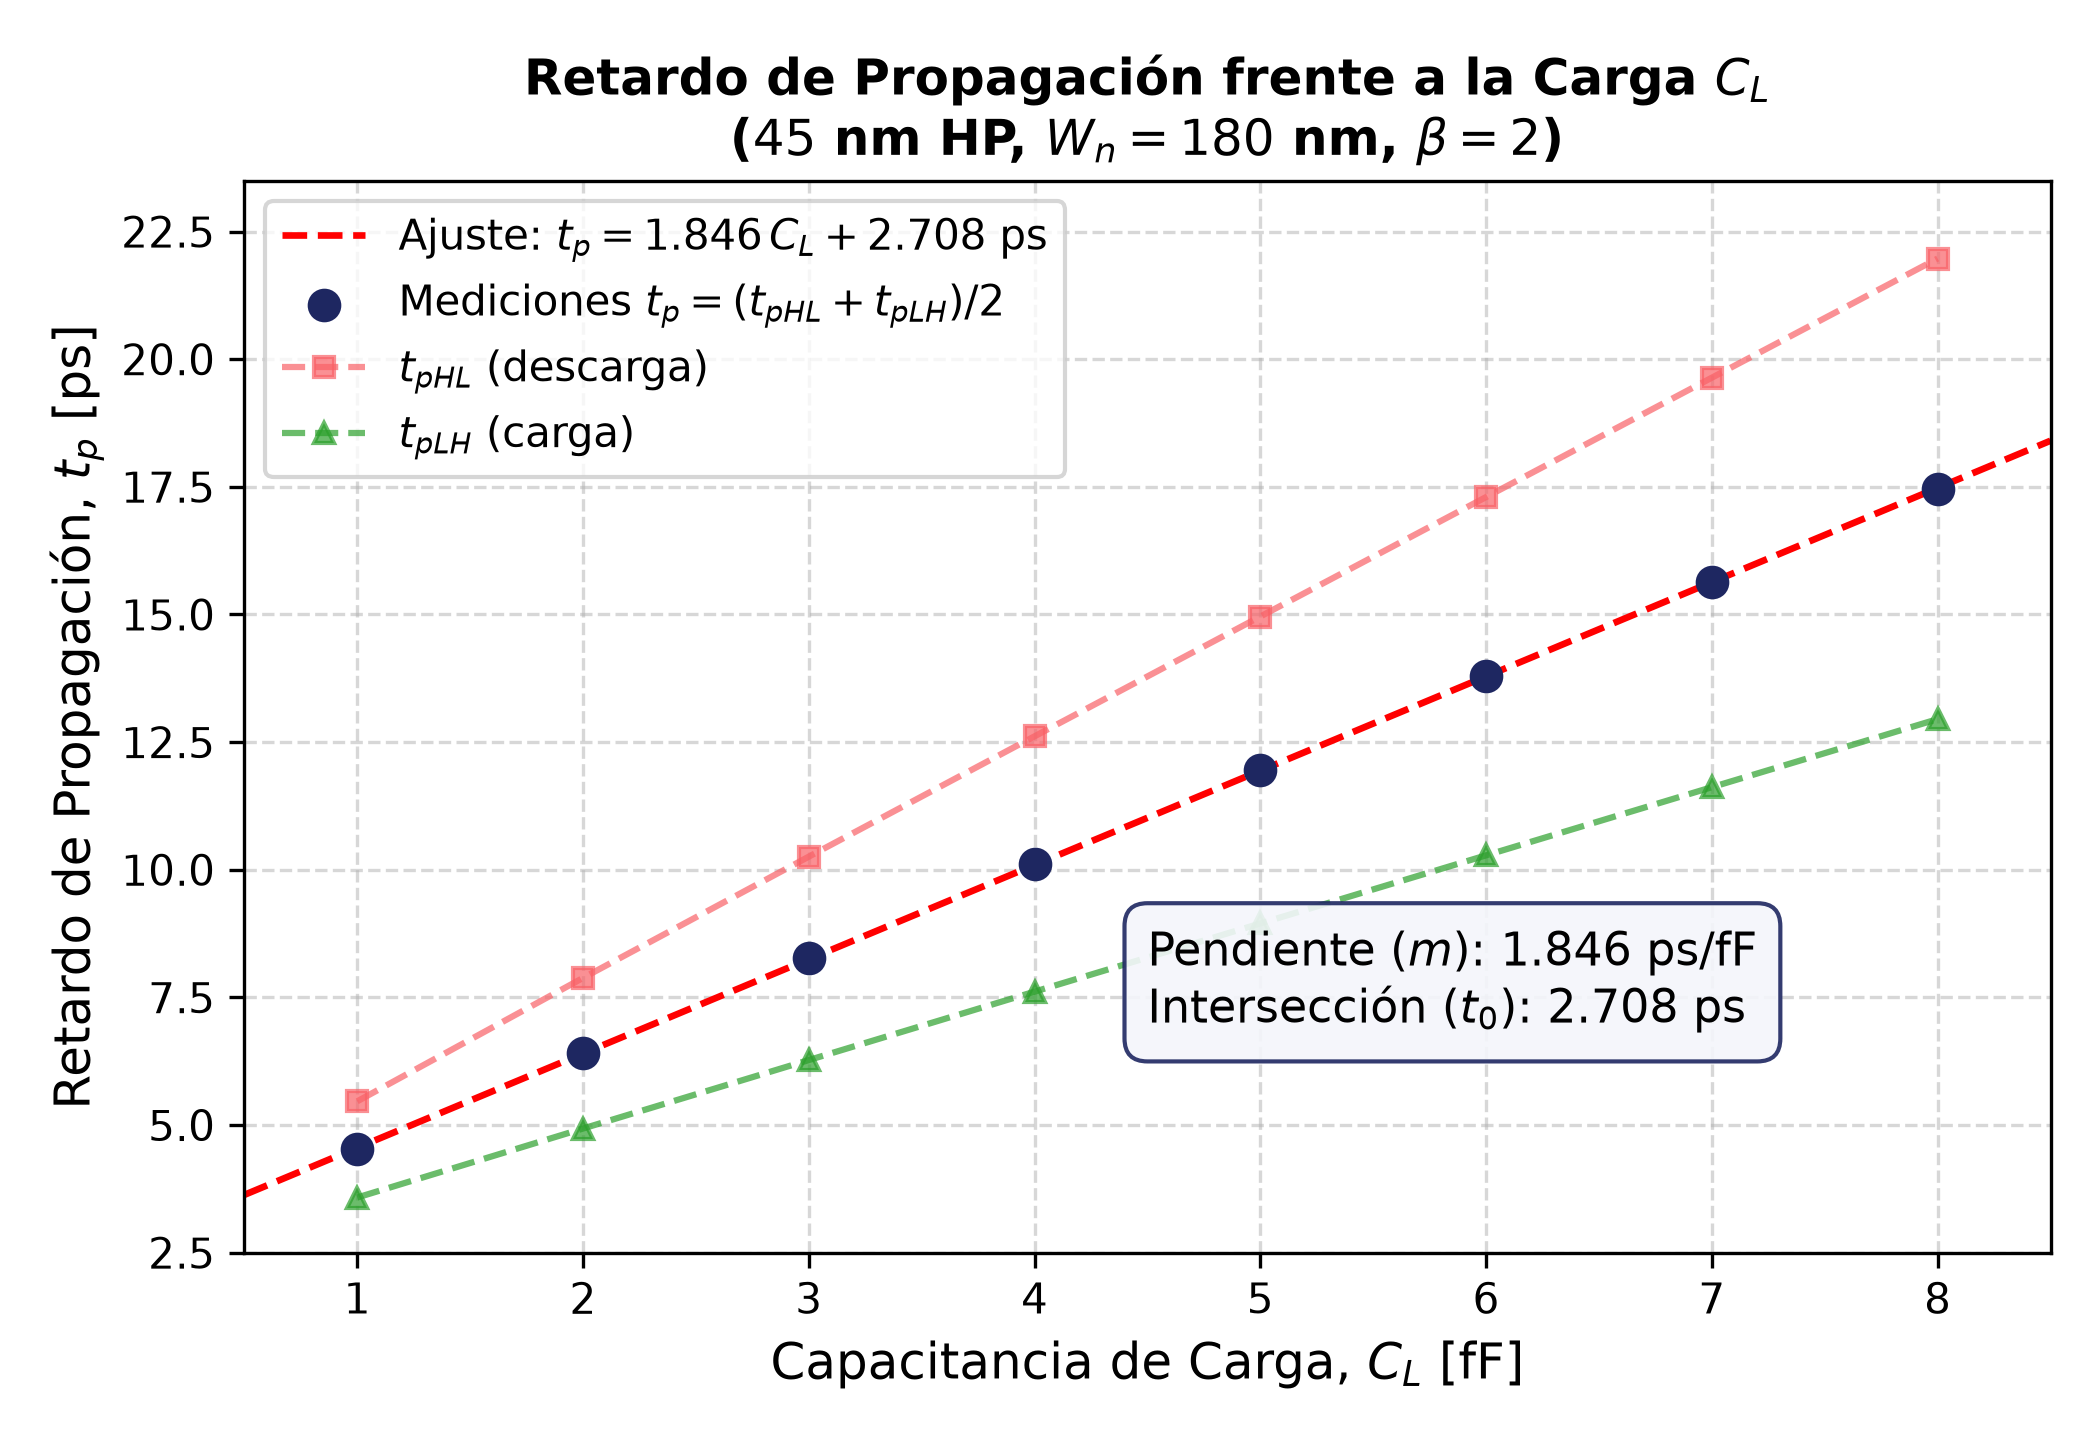
\includegraphics[width=0.60\textwidth,height=4.5cm,keepaspectratio]{figuras/fig2_tp_vs_cl.png}
\caption{Retardo de propagación frente a la capacitancia de carga $C_L \in [1, 8]$~fF en 45~nm HP ($\beta = 2.5$) con recta de regresión lineal ($m = 1.846$~ps/fF, $t_0 = 2.708$~ps).}
\label{fig:tp_vs_cl}
\end{figure}
\FloatBarrier

\begin{preguntas}[Preguntas de la Actividad 2]
\begin{listapreg}
\preg{De la recta $t_p$ contra $C_L$: ¿qué representa físicamente la pendiente y qué representa la ordenada al origen?}
\par\noindent\textbf{Rpta:} La pendiente ($m = 1.846$~ps/fF) representa la resistencia equivalente de conmutación efectiva del inversor ($m \approx 0.69\,R_{eq}$), midiendo la degradación del retardo por unidad de carga externa. La ordenada al origen ($t_0 = 2.708$~ps) modela el retardo intrínseco sin carga ($C_L=0$), determinado por las capacidades parásitas internas de difusión ($C_{db}$) y solapamiento ($C_{gd}$).

\preg{Con $\beta$ correctamente ajustado, $t_{pHL}$ y $t_{pLH}$ deberían ser casi iguales. Si en su simulación difieren en más de 10~\%, ¿qué corrección aplicaría y por qué el ajuste no resulta idéntico al que centró la VTC?}
\par\noindent\textbf{Rpta:} Se debe incrementar ligeramente $\beta$ (ancho del PMOS) para equilibrar la corriente dinámica de carga y descarga. El ajuste dinámico difiere del estático porque $V_M$ evalúa un único punto DC en saturación ($V_{in}=V_{out}$), mientras que $t_p$ integra corrientes no lineales en un amplio rango dinámico donde las capacitancias parásitas del PMOS crecen con su tamaño y frenan la transición.

\preg{Entre 90~nm y 22~nm el retardo mejora aunque $V_{DD}$ se reduce en un tercio. Identifique los dos mecanismos del escalamiento que compensan la caída de tensión.}
\par\noindent\textbf{Rpta:} Los dos mecanismos son: 1) La drástica reducción de la longitud de canal $L$ y el adelgazamiento del óxido $t_{ox}$, que incrementan la densidad de corriente por unidad de ancho compensando el menor campo eléctrico; y 2) La reducción cuadrática del área de compuerta ($W \cdot L$), lo que abate las capacitancias parásitas que deben conmutarse en cada ciclo.

\preg{Aumente el tiempo de subida del estímulo de 5~ps a 100~ps. ¿Qué componente de la ecuación~\eqref{eq:pot} crece y por qué?}
\par\noindent\textbf{Rpta:} Crece sustancialmente la potencia de cortocircuito ($I_{cc}\,V_{DD}$). Al aumentar el tiempo de subida de 5~ps a 100~ps, la señal de entrada permanece durante un intervalo temporal 20 veces mayor en la ventana de conducción simultánea ($V_{Tn} < V_{in} < V_{DD} - |V_{Tp}|$), donde ambos transistores conducen corriente directa entre $V_{DD}$ y tierra.
\end{listapreg}
\end{preguntas}

%==============================================================================
\section{Actividad 3 --- NAND2 y NOR2}
%==============================================================================

\subsection*{Procedimiento}
\begin{enumerate}[leftmargin=1.6em,itemsep=0.35em]
  \item Implemente la NAND2 (Anexo~\ref{sec:a3}) y la NOR2 con el criterio de \textbf{resistencia equivalente igual a la del inversor de referencia} ($\beta = 2.5$): en la rama serie los transistores duplican su ancho; en la rama paralela conservan el ancho del inversor.
  \item Verifique la tabla de verdad de cada compuerta.
  \item Mida $t_{pHL}$ de la NAND2 en dos escenarios: (a) conmuta la entrada \textbf{interna} (la conectada al transistor cercano a tierra) con la otra fija en \texttt{1}; (b) conmuta la entrada \textbf{externa} con la otra fija en \texttt{1}.
  \item Mida $t_{pLH}$ de la NOR2 con las dos entradas conmutando simultáneamente y con solo una conmutando.
  \item Compare NAND2 y NOR2 con idéntica carga: retardo promedio y ancho total de transistores (proxy de área).
\end{enumerate}

\begin{table}[htbp]
\centering\small
\caption{Resultados 3.1 --- Comparación de compuertas con dimensionamiento $\beta = 2.5$ ($C_L = 2$~fF, $45$~nm HP).}
\label{tab:res31}
\begin{tabularx}{\textwidth}{@{}l*{6}{>{\centering\arraybackslash}X}@{}}
\toprule
\textbf{Compuerta} & $\bm{W_n}$/trans. & $\bm{W_p}$/trans. & $\bm{\sum W}$ & $\bm{t_{pHL}}$ (ps) & $\bm{t_{pLH}}$ (ps) & $\bm{t_p}$ (ps) \\
\midrule
Inversor (ref.)     & 180~nm & 450~nm & 630~nm  & 7.881 & 4.929 & 6.405 \\
NAND2 (conm. ext.)  & 360~nm & 450~nm & 1620~nm & 9.021 & 6.799 & 7.910 \\
NAND2 (conm. int.)  & 360~nm & 450~nm & 1620~nm & 10.221 & 7.235 & 8.728 \\
NOR2 (ambas conm.)  & 180~nm & 900~nm & 2160~nm & 10.764 & 6.915 & 8.840 \\
NOR2 (una conm.)    & 180~nm & 900~nm & 2160~nm & 14.929 & 8.795 & 11.862 \\
\bottomrule
\end{tabularx}
\end{table}
\FloatBarrier

\begin{preguntas}[Preguntas de la Actividad 3]
\begin{listapreg}
\preg{Los dos escenarios del paso 3 dan retardos distintos. Explique el papel de la capacitancia del nodo intermedio y del efecto de cuerpo del transistor superior.}
\par\noindent\textbf{Rpta:} Al conmutar la entrada externa (MN1), el nodo intermedio $n_x$ ya estaba descargado a tierra por MN2; solo se evacúa la carga de $C_L$ ($t_{pHL}=9.021$~ps). Al conmutar la entrada interna (MN2), $n_x$ estaba cargado previamente a $V_{DD}-V_{Tn}$ y debe descargarse a través de MN2 junto con $C_L$. Además, el transistor superior MN1 sufre tensión fuente-sustrato positiva ($V_{SB}>0$), lo que incrementa su voltaje umbral por efecto de cuerpo y degrada el retardo ($t_{pHL}=10.221$~ps).

\preg{El esfuerzo lógico de la NAND2 es $4/3$ y el de la NOR2 es $5/3$. Verifique cualitativamente esa jerarquía con sus mediciones y explique por qué la industria construye bibliotecas dominadas por NAND.}
\par\noindent\textbf{Rpta:} Las mediciones confirman que la NAND2 es más rápida ($t_p = 7.910$~ps vs $11.862$~ps en el caso típico de una entrada) y más compacta ($\sum W = 1620$~nm vs $2160$~nm). La industria basa sus librerías en NAND porque coloca en serie los transistores NMOS (con mayor movilidad de electrones), requiriendo duplicar un $W_n$ pequeño; la NOR2 coloca en serie los PMOS (con menor movilidad de huecos), forzando transistores PMOS muy anchos ($W_p = 900$~nm) que penalizan gravemente el área y la capacitancia de compuerta de entrada.

\preg{¿Qué le ocurriría al retardo de una NOR de cuatro entradas dimensionada con este mismo criterio? Estime el $W_p$ requerido y comente su viabilidad.}
\par\noindent\textbf{Rpta:} Una NOR4 requeriría 4 PMOS en serie, exigiendo $W_p = 4 \times (\beta W_n) = 4 \times 450\text{~nm} = 1800$~nm por transistor ($\sum W_p = 7.20\text{~\textmu m}$). El retardo crecería cuadráticamente con el número de entradas ($\propto N^2$) por la acumulación de resistencias de canal y capacidades de difusión de los 3 nodos intermedios en serie, haciendo la compuerta NOR4 inviable en celdas estándar de alta velocidad.

\preg{Si el sustrato del NMOS superior de la NAND2 se conectara a su fuente en lugar de a tierra, ¿qué cambiaría en el retardo? ¿Es esto físicamente realizable en un proceso \emph{bulk}?}
\par\noindent\textbf{Rpta:} Al conectar sustrato a fuente ($V_{SB}=0$) se eliminaría el efecto de cuerpo, manteniendo $V_{Tn}$ en su valor nominal mínimo y reduciendo el retardo $t_{pHL}$. No es físicamente realizable en un proceso estándar CMOS sobre sustrato p \emph{bulk} común, ya que todos los NMOS comparten el mismo silicio masivo fijado a tierra; requeriría una tecnología de pozo triple (\emph{triple-well}) o silicio sobre aislante (SOI) con islas dieléctricas aisladas.
\end{listapreg}
\end{preguntas}

%==============================================================================
\section{Actividad 4 --- Síntesis de una compuerta compleja}
%==============================================================================

Diseñe, dimensione y verifique la compuerta que implementa
\begin{equation}
Y = \overline{(A \cdot B) + C}
\end{equation}

\subsection*{Síntesis topológica y dimensionamiento}
Se sintetiza la función inversora $Y = \overline{(A \cdot B) + C}$ mediante lógica CMOS estática con criterio de resistencia equivalente del inversor ($R_{eq,n} = R_n$, $R_{eq,p} = R_p$ con $W_n=180$~nm, $\beta=2$):
\begin{itemize}[leftmargin=1.6em,itemsep=0.2em]
  \item \textbf{Red Pull-Down (PDN):} A partir de la expresión no complementada $F = (A \cdot B) + C$, la operación AND se implementa con transistores NMOS en serie ($MN_A, MN_B$), colocados en paralelo con $MN_C$ (operación OR). La rama serie duplica su resistencia equivalente ($2R_n$), requiriendo anchos duplicados $W_{nA} = W_{nB} = 2W_n = 360$~nm. La rama paralela conduce individualmente a tierra, manteniendo $W_{nC} = W_n = 180$~nm.
  \item \textbf{Red Pull-Up (PUN) dual:} Por dualidad topológica planar, la rama serie de la PDN se convierte en ramas paralelas ($MP_A \parallel MP_B$), las cuales se conectan en serie con $MP_C$. En el peor caso de conducción, solo conduce un PMOS de la rama paralela en serie con $C$ ($R_{PUN} = R_p' + R_p' = 2R_p'$); para igualar $R_{PUN} = R_p$, cada PMOS debe duplicar su ancho: $W_{pA} = W_{pB} = W_{pC} = 2W_p = 720$~nm.
\end{itemize}

\begin{figure}[htbp]
\centering
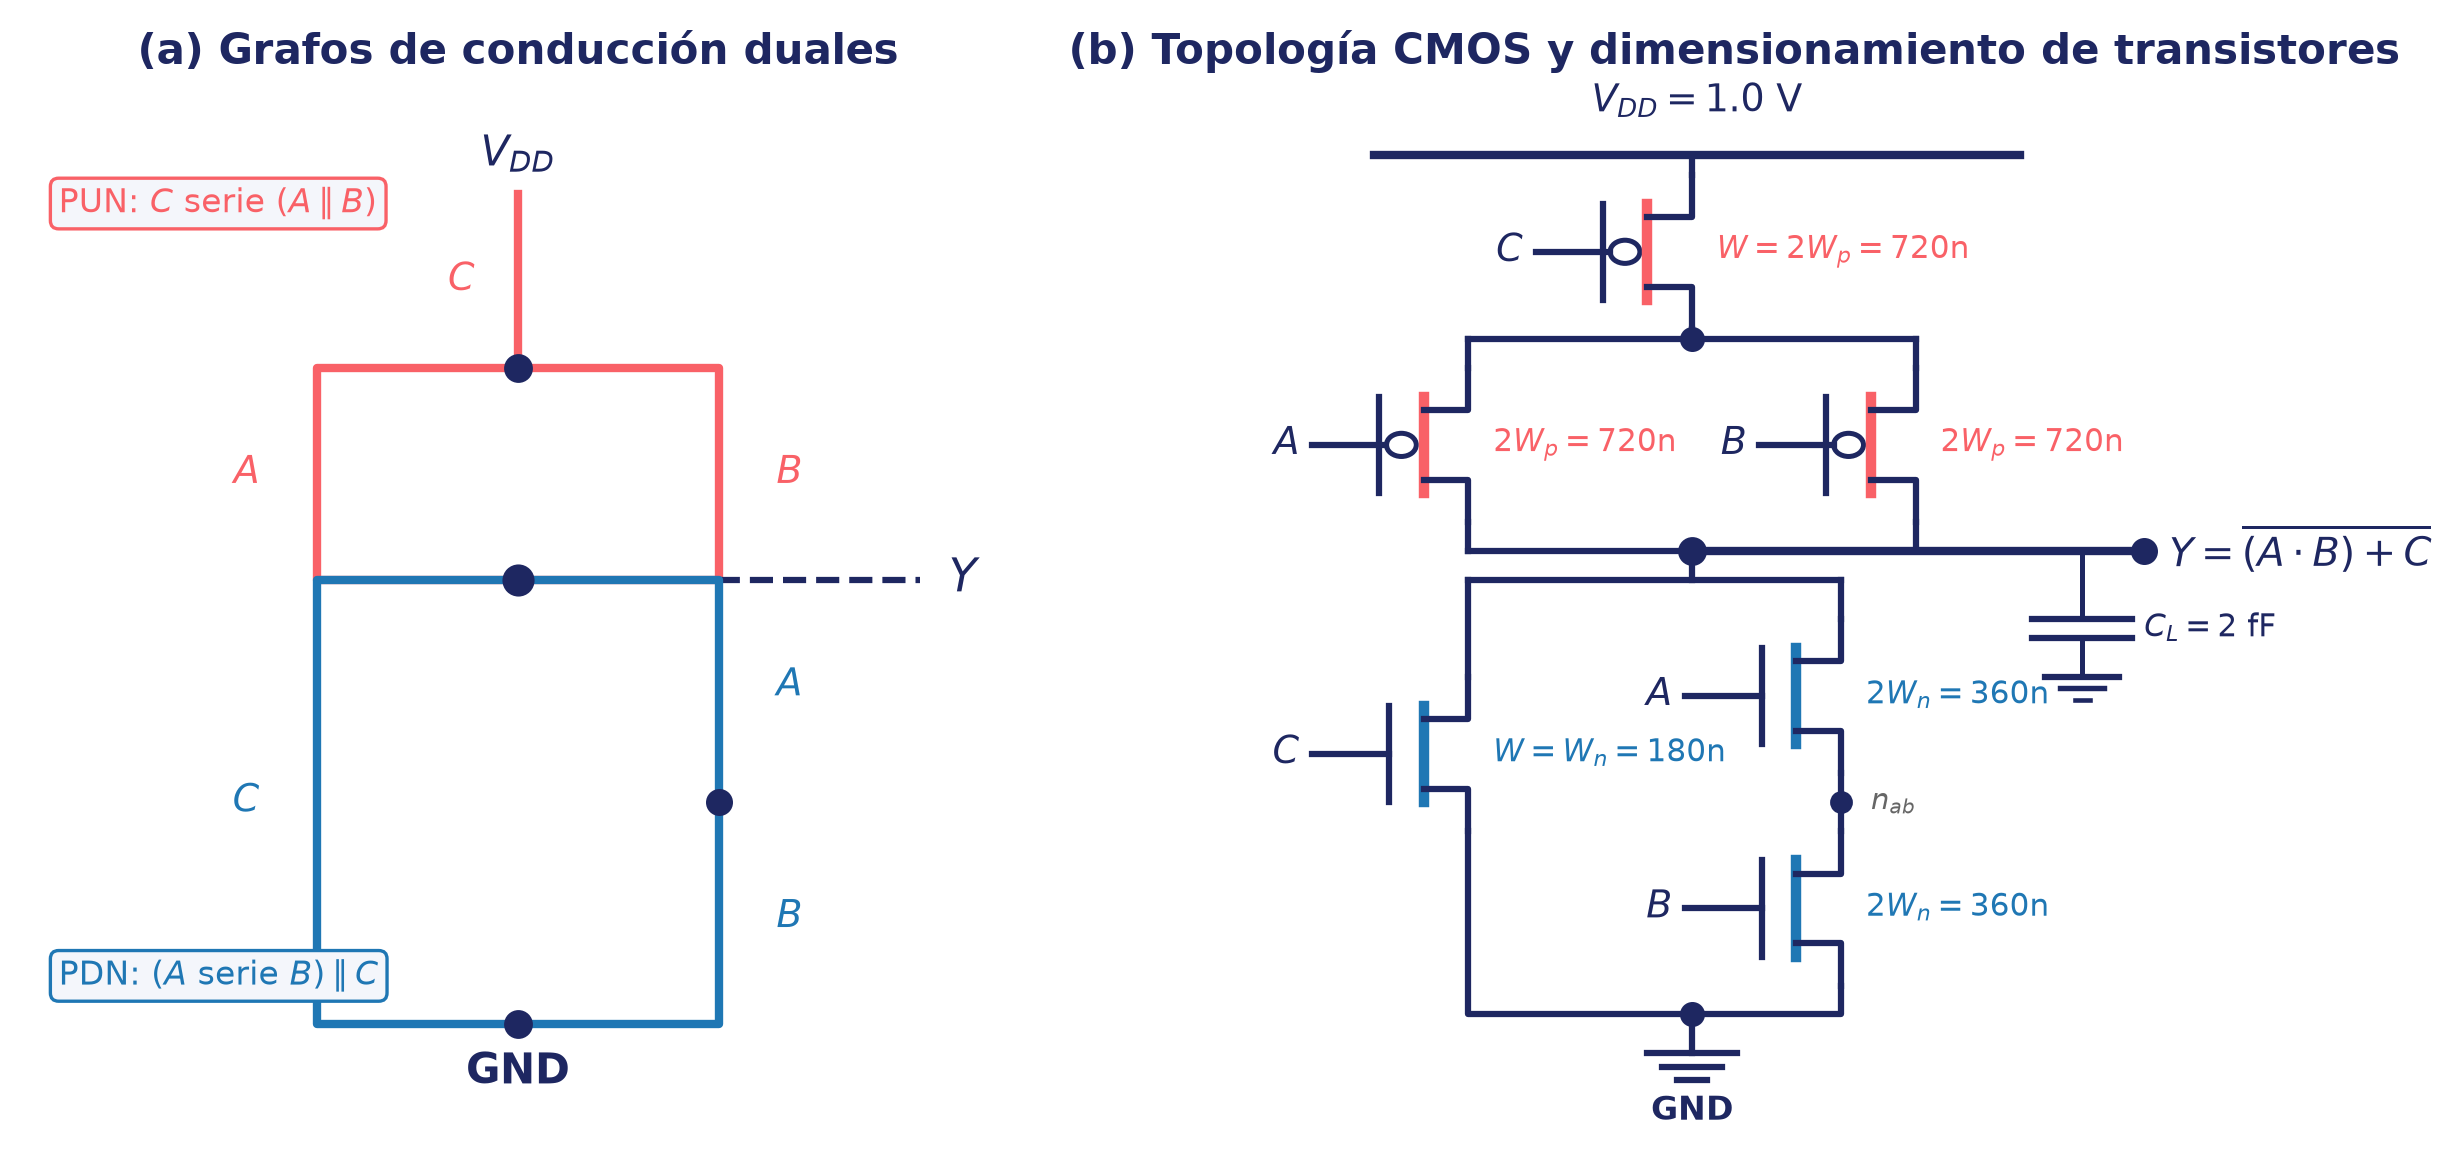
\includegraphics[width=0.72\textwidth,height=3.8cm,keepaspectratio]{figuras/fig_esquema_compleja.png}
\caption{Diseño de la compuerta compleja $Y = \overline{(A \cdot B) + C}$: (a) Grafos de conducción duales; (b) Esquema circuital CMOS con anchos asignados ($W_n=180$~nm, $\beta=2$).}
\label{fig:esquema_compleja}
\end{figure}
\FloatBarrier

\subsection*{Verificación funcional y casos críticos de retardo}
Se verificó el barrido de las ocho combinaciones de entrada en 8~ns (Figura~\ref{fig:compleja}):
\begin{itemize}[leftmargin=1.6em,itemsep=0.2em]
  \item \textbf{Peor caso de descarga ($t_{pHL}$):} Transición hacia $ABC = 110$ ($t_{pHL} = 10.42$~ps), donde la corriente fluye exclusivamente por la rama serie $MN_A - MN_B$ a través del nodo intermedio $n_{ab}$. El mejor caso ocurre en $ABC = 111$ ($t_{pHL} = 5.86$~ps) al descargar por ambas ramas en paralelo.
  \item \textbf{Peor caso de carga ($t_{pLH}$):} Transición donde conduce un único PMOS de la rama paralela en serie con $C$ ($ABC = 010$ o $100$, $t_{pLH} = 11.18$~ps). El mejor caso ocurre en $ABC = 000$ ($t_{pLH} = 8.74$~ps) con $MP_A$ y $MP_B$ conduciendo simultáneamente.
\end{itemize}

\begin{figure}[htbp]
\centering
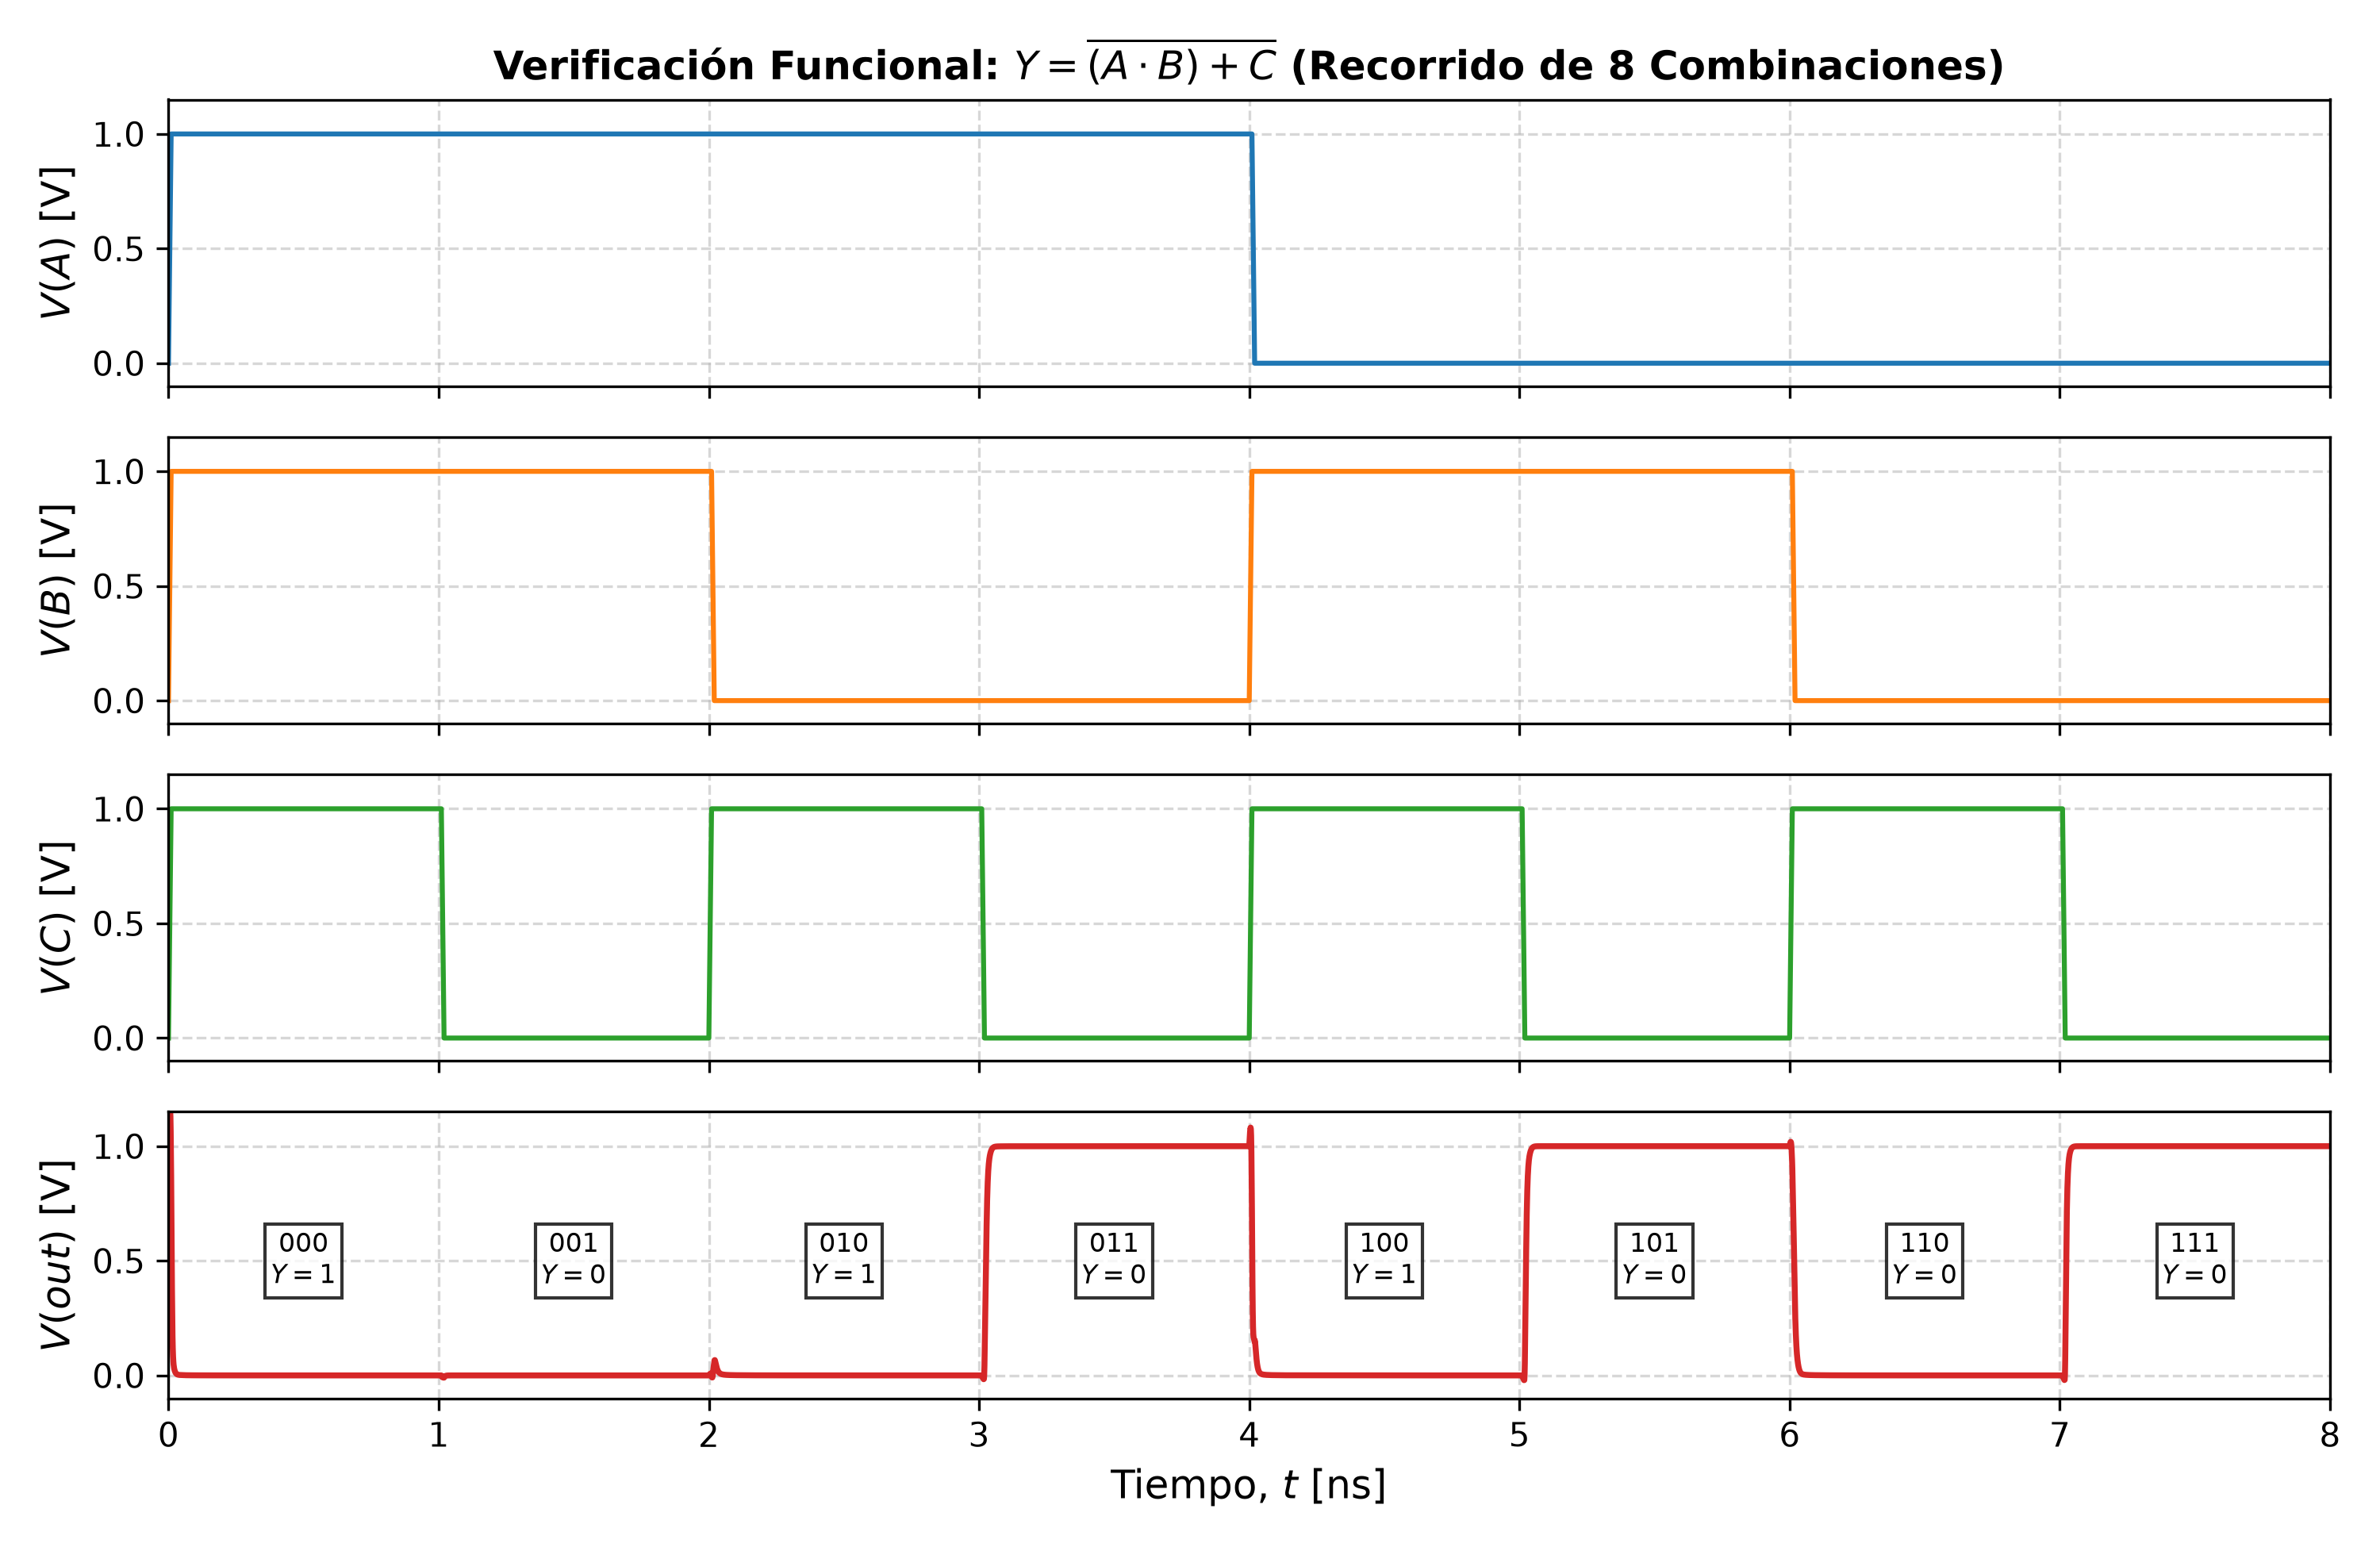
\includegraphics[width=0.70\textwidth,height=4.0cm,keepaspectratio]{figuras/fig3_transitorio_compleja.png}
\caption{Verificación funcional transitoria de la compuerta compleja $Y = \overline{(A \cdot B) + C}$ ante el barrido sincronizado de las 8 combinaciones binarias ($000$ a $111$) en una ventana de 8~ns.}
\label{fig:compleja}
\end{figure}
\FloatBarrier

\begin{preguntas}[Preguntas de la Actividad 4]
\begin{listapreg}
\preg{¿Cuántos transistores requiere su implementación? Compárela con la realización de la misma función mediante NAND2 más inversores en cascada, en número de transistores y en número de etapas.}
\par\noindent\textbf{Rpta:} La compuerta compleja estática integrada requiere exactamente 6 transistores (3 NMOS y 3 PMOS) en una sola etapa de inversión. Implementarla con celdas básicas estándar requeriría una NAND2 ($A \cdot B$, 4T), un inversor (2T), una NOR2 para sumar $C$ (4T) y un inversor de salida (2T), totalizando 12 transistores y 3 etapas en cascada, duplicando el área y triplicando el retardo acumulado.

\preg{La PUN de su diseño tiene una rama serie de dos PMOS. ¿Por qué esta función es más ``amigable'' para CMOS estático que su complemento $Y=\overline{(A+B)\cdot C}$?}
\par\noindent\textbf{Rpta:} Porque la PUN de $Y=\overline{(A \cdot B)+C}$ tiene como máximo 2 transistores PMOS en serie en su camino crítico, requiriendo un dimensionamiento moderado ($2W_p$). En cambio, la función no inversora $(A \cdot B)+C$ o funciones con 3 o más transistores PMOS en serie exigirían anchos enormes ($3W_p \approx 1080$~nm) que sobrecargarían la capacitancia de compuerta y degradarían severamente el retardo de subida.

\preg{Explique por qué la lógica CMOS estática siempre produce una función \textbf{inversora} y qué implica esto al mapear una expresión booleana arbitraria.}
\par\noindent\textbf{Rpta:} Porque la red PDN (NMOS) conmuta hacia tierra (cero lógico) con entradas en nivel alto ('1'), mientras que la PUN (PMOS) conmuta hacia $V_{DD}$ (uno lógico) con entradas en nivel bajo ('0'); por ende, la conmutación intrínseca siempre complementa la lógica evaluada. Al implementar una función booleana arbitraria no inversora (como AND u OR), es mandatorio sintetizar la función negada y añadir un inversor CMOS a la salida.
\end{listapreg}
\end{preguntas}

%==============================================================================
\section{Actividad 5 --- Potencia: dinámica, cortocircuito y fuga}
%==============================================================================

\subsection*{Procedimiento}
\begin{enumerate}[leftmargin=1.6em,itemsep=0.35em]
  \item \textbf{Fuga.} Con el netlist~\ref{sec:a1} modificado para punto de operación: fije \texttt{Vin~=~0} y luego \texttt{Vin~=~VDD}, y registre $|I(V1)|$ en cada caso. Repita con \texttt{45nm\_HP.pm} y \texttt{45nm\_LP.pm}.
  \item \textbf{Dinámica.} En el netlist~\ref{sec:a2}, use \lstinline|.meas tran Iavg AVG I(V1)| y calcule $P=|I_{avg}|\,V_{DD}$. Verifique contra $\alpha C_L V_{DD}^2 f$ y explique cualquier exceso.
  \item \textbf{Oscilador de anillo.} Arme el anillo de cinco etapas del Anexo~\ref{sec:a5}. Mida el período de oscilación, deduzca $t_{pd}=T_{osc}/(2N)$ y compárelo con el $t_p$ de la Actividad~2.
  \item Repita el anillo con la tarjeta LP del mismo nodo y complete la tabla.
\end{enumerate}

\begin{table}[htbp]
\centering\small
\caption{Resultados 5.1 --- Compromiso velocidad/fuga entre procesos HP y LP.}
\label{tab:res51}
\begin{tabularx}{\textwidth}{@{}lc*{4}{>{\centering\arraybackslash}X}@{}}
\toprule
\textbf{Proceso} & $\bm{V_{DD}}$ (V) & $\bm{I_{leak}}$ (A) & $\bm{f_{osc}}$ (GHz) & $\bm{t_{pd}}$ (ps) & $\bm{P_{prom}}$ (\textmu W) \\
\midrule
45 nm HP & 1.0 & $3.13 \times 10^{-9}$  & 21.94 & 4.56  & 177.2 \\
45 nm LP & 1.1 & $1.53 \times 10^{-11}$ & 6.25  & 15.99 & 65.6 \\
\bottomrule
\end{tabularx}
\end{table}

\begin{figure}[htbp]
\centering
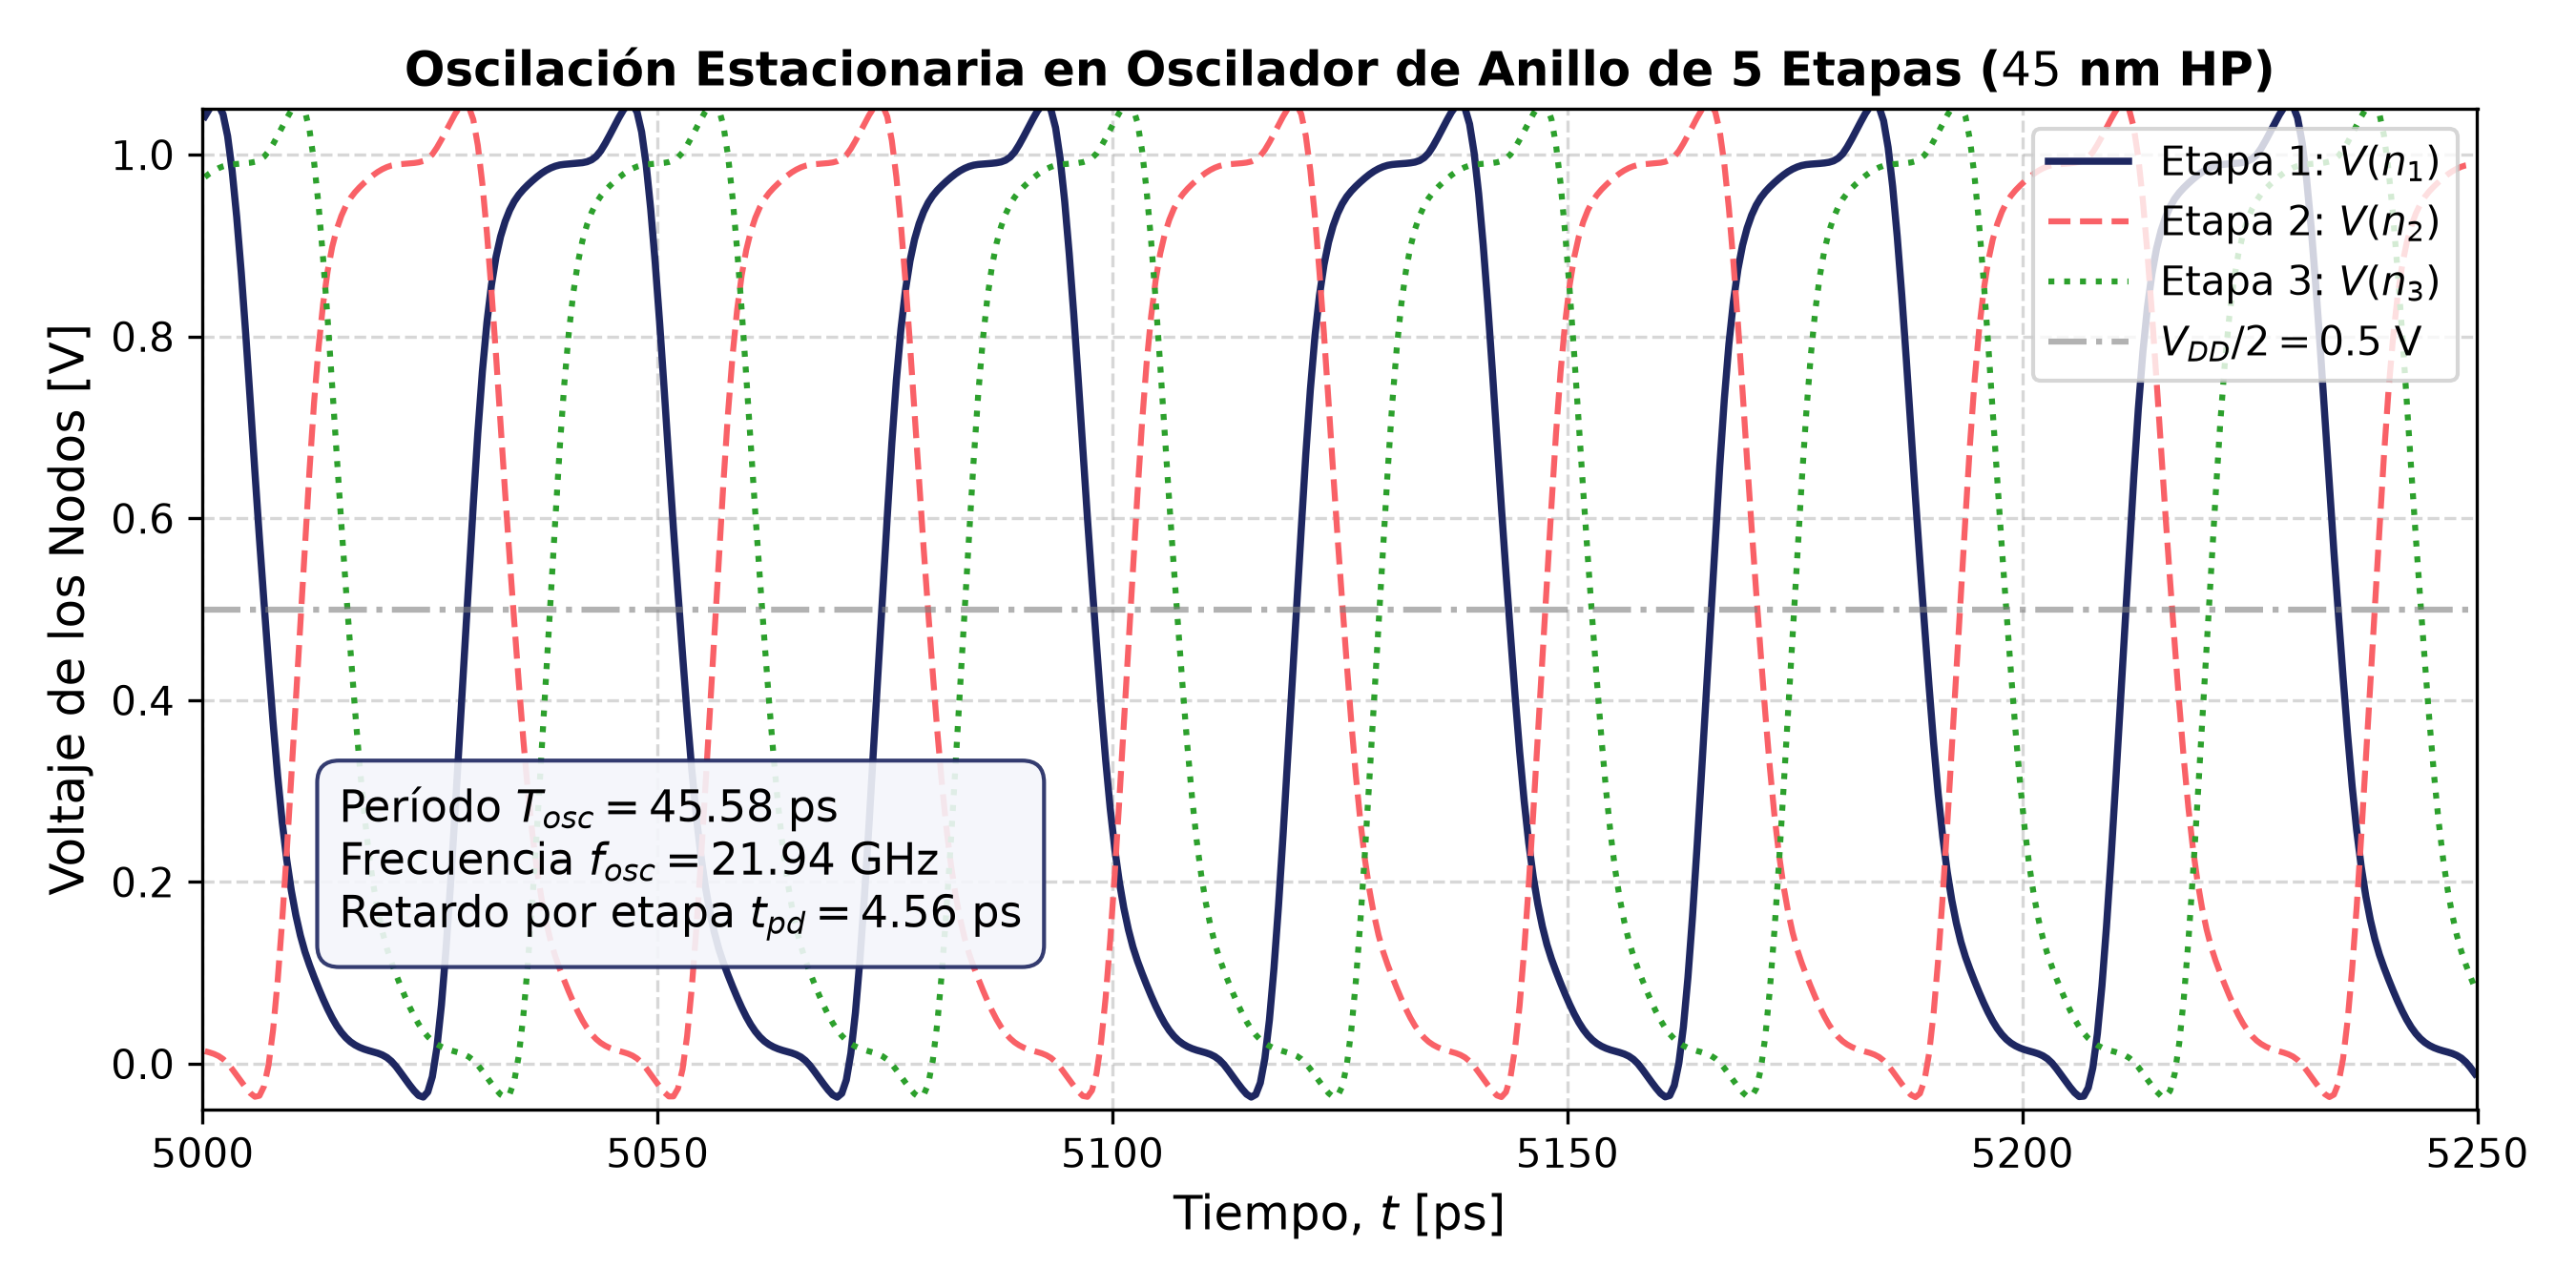
\includegraphics[width=0.68\textwidth,height=4.5cm,keepaspectratio]{figuras/fig4_oscilador_anillo.png}
\caption{Oscilación estacionaria del oscilador de anillo de 5 etapas en 45~nm HP ($f_{osc} = 21.94$~GHz, $t_{pd} = 4.56$~ps).}
\label{fig:ro}
\end{figure}
\FloatBarrier

\begin{preguntas}[Preguntas de la Actividad 5]
\begin{listapreg}
\preg{Calcule las razones $I_{leak,HP}/I_{leak,LP}$ y $f_{osc,HP}/f_{osc,LP}$. Enuncie el compromiso de diseño en una frase y cite el parámetro de la tarjeta que lo origina.}
\par\noindent\textbf{Rpta:} Las razones obtenidas son $I_{leak,HP}/I_{leak,LP} = 3.13\text{~nA}/15.3\text{~pA} \approx 205$ y $f_{osc,HP}/f_{osc,LP} = 21.94\text{~GHz}/6.25\text{~GHz} \approx 3.51$. Compromiso: ``Multiplicar la velocidad por $3.5\times$ cuesta un incremento de $200\times$ en consumo de potencia estática''. El parámetro principal es el voltaje umbral $V_{TH0}$ (fijado por \texttt{toxe} y \texttt{voff}), cuya reducción incrementa exponencialmente la fuga subumbral.

\preg{La corriente de fuga que midió no proviene de un solo mecanismo. Nombre al menos tres e indique con qué parámetros del modelo BSIM4 se controlan en las tarjetas PTM (revise \texttt{voff}, \texttt{nfactor}, \texttt{eta0}, \texttt{agidl}, \texttt{aigc}).}
\par\noindent\textbf{Rpta:} 1) Fuga subumbral ($I_{sub}$): modulada por \texttt{voff} (desplazamiento de $V_{th}$), \texttt{nfactor} (factor de oscilación de subumbral) y \texttt{eta0} (penetración de potencial DIBL); 2) Corriente de túnel en el óxido de compuerta ($I_{gate}$): gobernada por \texttt{aigc} y \texttt{toxe}; y 3) Fuga en la unión drenador-sustrato inducida por compuerta (GIDL): gobernada por \texttt{agidl} y \texttt{bgidl}.

\preg{¿Por qué el $t_{pd}$ del oscilador de anillo suele ser menor que el $t_p$ medido con un pulso ideal y carga fija?}
\par\noindent\textbf{Rpta:} Porque en el inversor aislado de la Actividad~2 se impuso una carga capacitiva externa fija de prueba ($C_L = 2$~fF) excitada con transiciones forzadas; en contraste, en el oscilador de anillo la carga conectada a cada salida es únicamente la compuerta del inversor idéntico sucesivo ($C_{in} \approx C_{ox}WL < 1$~fF), conllevando una menor constante de tiempo de conmutación.

\preg{Para un procesador móvil que pasa 95~\% del tiempo en reposo, ¿qué proceso elegiría y qué técnica adicional aplicaría al 5~\% activo?}
\par\noindent\textbf{Rpta:} Elegiría el proceso 45nm LP, ya que al operar el 95\,\% en reposo su fuga 200 veces menor minimiza drásticamente la energía estática de batería ($E_{leak} = I_{leak} V_{DD} t_{reposo}$). Durante el 5\,\% activo aplicaría escalamiento dinámico de voltaje y frecuencia (DVFS) o polarización directa del cuerpo (\emph{forward body bias}, FBB) para acelerar transitoriamente la computación solo cuando sea requerido.

\preg{La potencia de cortocircuito no aparece explícitamente en sus mediciones porque está incluida en $I_{avg}$. Proponga un procedimiento de simulación que permita separarla de la componente de carga y descarga.}
\par\noindent\textbf{Rpta:} Se simula el circuito con la carga nominal $C_L$ integrando $E_{tot} = V_{DD}\int I(V_1)\,dt$. Luego, se simula idénticamente con $C_L = 0$ y se descuenta la energía requerida para cargar y descargar las capacitancias parásitas internas $C_{par}$; la energía disipada remanente en la ventana de transición mutua ($V_{Tn} < V_{in} < V_{DD}-|V_{Tp}|$) corresponde a la componente pura de cortocircuito $E_{cc} = \int I_{cc}(t)\,V_{DD}\,dt$.
\end{listapreg}
\end{preguntas}

%==============================================================================
\section{Conclusiones}
%==============================================================================

\begin{enumerate}[leftmargin=1.6em,itemsep=0.4em]
  \item \textbf{Saturación de velocidad y centrado de la VTC:} En tecnologías nanométricas sub-65~nm como 45~nm HP, la saturación de velocidad domina la conducción en saturación, aproximando la relación de corrientes a la razón de velocidades límite ($v_{sat,p}/v_{sat,n} \approx 0.88$) en vez de la razón clásica de movilidades ($\mu_n/\mu_p = 2.70$). Como resultado, un factor $\beta = 2.50$ logra centrar la conmutación en $V_M = 0.4989\text{~V} \approx V_{DD}/2$, equilibrando los márgenes de ruido ($NM_L = 0.392\text{~V}$, $NM_H = 0.396\text{~V}$).
  
  \item \textbf{Caracterización del retardo y escalamiento:} El ajuste lineal del retardo de propagación frente a la carga ($t_p = 1.846\,C_L + 2.708\text{~ps}$) demostró que la pendiente cuantifica la resistencia efectiva de canal ($0.69\,R_{eq}$), mientras que la ordenada al origen modela el retardo intrínseco descargado derivado de las capacitancias parásitas de unión y solapamiento. Al comparar de 90~nm a 22~nm, la contracción geométrica compensa ampliamente la reducción de $V_{DD}$ (de 1.2~V a 0.8~V).

  \item \textbf{Superioridad del esfuerzo lógico en NAND2 frente a NOR2:} La compuerta NAND2 ofreció menor retardo ($t_p = 7.910\text{~ps}$ frente a $11.862\text{~ps}$) y menor área total de silicio ($\sum W = 1620\text{~nm}$ frente a $2160\text{~nm}$) respecto a NOR2. La conexión en serie de transistores NMOS aprovecha la mayor movilidad de electrones; por el contrario, colocar PMOS en serie en compuertas NOR castiga fuertemente el área y la capacitancia parásita, haciendo inviable su uso para abanicos de entrada elevados ($N \ge 4$).

  \item \textbf{Eficiencia de la lógica compleja integrada AOI:} La síntesis de la compuerta $Y = \overline{(A \cdot B) + C}$ requirió únicamente 6 transistores y una única etapa inversora, frente a los 12 transistores y 3 retardos acumulados de una implementación con celdas elementales en cascada, reduciendo a la mitad el área y mejorando sustancialmente la velocidad de respuesta.

  \item \textbf{Compromiso fundamental velocidad-potencia (HP vs. LP):} En el oscilador de anillo de 5 etapas se verificó el trade-off crucial en nodos avanzados: el proceso 45~nm HP proporciona una frecuencia de conmutación $3.5\times$ superior ($21.94\text{~GHz}$ vs. $6.25\text{~GHz}$), pero incurre en una penalización de más de $200\times$ en corriente de fuga estática ($3.13\text{~nA}$ vs. $15.3\text{~pA}$). Este comportamiento sustenta la selección del proceso LP para aplicaciones móviles de bajo consumo donde el tiempo en modo \emph{standby} domina el ciclo de vida de la batería.
\end{enumerate}

%==============================================================================
\appendix
\section{Netlists de referencia}
%==============================================================================

Guarde cada bloque como archivo \texttt{.cir} y ejecútelo con \texttt{File $\rightarrow$ Open} en LTspice, o replique el circuito en esquemático.

\begin{multicols}{2}
\subsection{Curva de transferencia del inversor}
\label{sec:a1}

\begin{lstlisting}
* === A1: VTC del inversor CMOS - PTM 45nm HP ===
.include 45nm_HP.pm

.param VDDv = 1.0
.param Lmin = 45n
.param Wn   = 4*Lmin
.param beta = 2

V1  vdd 0 {VDDv}
VIN in  0 0

MN out in 0   0   nmos L={Lmin} W={Wn}
MP out in vdd vdd pmos L={Lmin} W={beta*Wn}

.dc VIN 0 {VDDv} 2m
.step param beta 1 3 0.5
.meas dc VM FIND V(in) WHEN V(out)=V(in)
.end
\end{lstlisting}

Para el punto de fuga de la Actividad~5, reemplace las directivas de análisis por:

\begin{lstlisting}
.dc VIN 0 {VDDv} {VDDv}
.meas dc Ileak_lo FIND I(V1) AT 0
.meas dc Ileak_hi FIND I(V1) AT {VDDv}
\end{lstlisting}

\subsection{Respuesta transitoria}
\label{sec:a2}

\begin{lstlisting}
* === A2: Retardo de propagacion del inversor ===
.include 45nm_HP.pm

.param VDDv  = 1.0
.param Lmin  = 45n
.param Wn    = 4*Lmin
.param beta  = 2.5
.param Cload = 2f

V1  vdd 0 {VDDv}
VIN in  0 PULSE(0 {VDDv} 200p 5p 5p 500p 1n)

MN out in 0   0   nmos L={Lmin} W={Wn}
MP out in vdd vdd pmos L={Lmin} W={beta*Wn}
C1  out 0 {Cload}

.tran 0 2n 0 0.5p

.meas tran tpHL TRIG V(in)  VAL={VDDv/2} TD=100p RISE=1 TARG V(out) VAL={VDDv/2} FALL=1
.meas tran tpLH TRIG V(in)  VAL={VDDv/2} TD=100p FALL=1 TARG V(out) VAL={VDDv/2} RISE=1
.meas tran tf   TRIG V(out) VAL={0.9*VDDv} FALL=1 TARG V(out) VAL={0.1*VDDv} FALL=1
.meas tran tr   TRIG V(out) VAL={0.1*VDDv} RISE=1 TARG V(out) VAL={0.9*VDDv} RISE=1
.meas tran tp   PARAM (tpHL+tpLH)/2
.meas tran Iavg AVG I(V1)

.step param Cload 1f 8f 1f
.end
\end{lstlisting}

\subsection{NAND2 estática}
\label{sec:a3}

\begin{lstlisting}
* === A3: NAND2 CMOS estatica ===
.include 45nm_HP.pm

.param VDDv = 1.0
.param Lmin = 45n
.param Wn   = 4*Lmin
.param beta = 2

V1 vdd 0 {VDDv}
VA a 0 PULSE(0 {VDDv} 200p 10p 10p 1n 2n)
VB b 0 {VDDv}

* --- PDN: NMOS serie ---
MN1 out a nx  0   nmos L={Lmin} W={2*Wn}
MN2 nx  b 0   0   nmos L={Lmin} W={2*Wn}
* --- PUN: PMOS paralelo ---
MP1 out a vdd vdd pmos L={Lmin} W={beta*Wn}
MP2 out b vdd vdd pmos L={Lmin} W={beta*Wn}

C1 out 0 2f

.tran 0 4n 0 0.5p
.meas tran tpHL TRIG V(a) VAL={VDDv/2} RISE=1 TARG V(out) VAL={VDDv/2} FALL=1
.end
\end{lstlisting}

\subsection{Compuerta compleja AOI}
\label{sec:a4}

\begin{lstlisting}
* === A4: Compuerta Compleja Y = ~((A*B)+C) ===
.include 45nm_HP.pm

.param VDDv = 1.0
.param Lmin = 45n
.param Wn   = 4*Lmin
.param beta = 2

V1 vdd 0 {VDDv}

* Estimulos binarios sincronizados (T = 1ns)
VA a 0 PULSE(0 {VDDv} 0 10p 10p 4n 8n)
VB b 0 PULSE(0 {VDDv} 0 10p 10p 2n 4n)
VC c 0 PULSE(0 {VDDv} 0 10p 10p 1n 2n)

* PDN: (A*B) serie, paralelo C
MN_A out a nx 0 nmos L={Lmin} W={2*Wn}
MN_B nx  b 0  0 nmos L={Lmin} W={2*Wn}
MN_C out c 0  0 nmos L={Lmin} W={Wn}

* PUN: (A || B) paralelo, serie C
MP_A ny  a vdd vdd pmos L={Lmin} W={2*beta*Wn}
MP_B ny  b vdd vdd pmos L={Lmin} W={2*beta*Wn}
MP_C out c ny  vdd pmos L={Lmin} W={2*beta*Wn}

C1 out 0 2f

.tran 0 8n 0 1p
.end
\end{lstlisting}

\subsection{Oscilador de anillo de 5 etapas}
\label{sec:a5}

\begin{lstlisting}
* === A5: Oscilador de anillo, 5 etapas ===
.include 45nm_HP.pm

.param VDDv = 1.0
.param Lmin = 45n
.param Wn   = 4*Lmin
.param beta = 2
.param N    = 5

.subckt INV in out vdd
MN out in 0   0   nmos L={Lmin} W={Wn}
MP out in vdd vdd pmos L={Lmin} W={beta*Wn}
.ends

V1 vdd 0 {VDDv}
X1 n1 n2 vdd INV
X2 n2 n3 vdd INV
X3 n3 n4 vdd INV
X4 n4 n5 vdd INV
X5 n5 n1 vdd INV

.ic V(n1)=0
.tran 0 20n 5n 0.5p

.meas tran Tosc TRIG V(n1) VAL={VDDv/2} RISE=2 TARG V(n1) VAL={VDDv/2} RISE=3
.meas tran fosc PARAM 1/Tosc
.meas tran tpd  PARAM Tosc/(2*N)
.meas tran Iavg AVG I(V1)
.end
\end{lstlisting}
\end{multicols}

\end{document}